\documentclass[conference]{IEEEtran}
\usepackage{cite}
\usepackage{amsmath,amssymb,amsfonts}
\usepackage{algorithmic}
\usepackage{float}
\usepackage[caption = false]{subfig}
\usepackage[final]{graphicx}
\usepackage{textcomp}
\usepackage{xcolor}
\def\BibTeX{{\rm B\kern-.05em{\sc i\kern-.025em b}\kern-.08em
    T\kern-.1667em\lower.7ex\hbox{E}\kern-.125emX}}
\graphicspath{{C:/Users/Terry/Desktop/Documents/MyLaTex/CSC 592 ABD - Term Paper/Report Images/}}

\begin{document}
\pagestyle{plain}
\title{Analysis of Radio Frequency Data utilizing Clustering Methods\\
}
\author{\IEEEauthorblockN{Terry R. Ferguson}
\IEEEauthorblockA{\textit{Computer Science and Statistics} \\
\textit{University of Rhode Island}\\
\textit{Kingston, RI 02881}\\
\textit{terry\_ferguson@uri.edu}}
}
\maketitle

\begin{abstract}
Determining channel availability in radio communications is a key enabler of cognitive radios. In this paper we review a popular and validated radio frequency data set (RadioML 2018) in an effort to determine if approaches associated with high dimensional reduction through clustering such as Uniform Manifold Approximation and Projection (UMAP) and Clustered Hierarchical Anomaly and Outlier Detection Algorithms (CHAODA) could provide additional opportunities in classification, anomaly detection or provide a reduction in uncertainty thus improving channel availability detection in cognitive radios. 
\end{abstract}

\begin{IEEEkeywords}
Spectrum Sensing, Channel Availability, Clustered Anomaly Detection
\end{IEEEkeywords}

\section{Introduction}
Cognitive radios are software defined radios that make autonomous decisions and can facilitate modern capabilities beyond that which has been historically provided; among them is the ability to negotiate an open channel to support communications from the available allocated radio spectrum or spectrum sensing.  This requires the transmitter to determine which channels are open and a receiver that can find the transmit channel across a number of available channels. The Federal Communications Commission in 2003 \cite{b1} proposed rulings that officially recognized the benefits of cognitive radios, specifically spectrum sensing; indicating how they could promote more effective use of the radio spectrum by recognizing unused parts or white spaces to support a coordinate adaptive communication. 
 
In planned communications transmitters and receivers can optimize the use of a shared set of channels without a coordination channel. Removing the need for coordination further promotes autonomy and allows for uncoordinated communications across a large set of channels or the potions of the radio spectrum as such spectrum sensing could benefit public safety for example; through the use of cognitive radio enabled unmanned aerial vehicles (UAV) that support rescue efforts or establishing communications after a disaster \cite{b2} as well as support military UAV applications \cite{b3} where the communications within a foreign airspace may not be cooperative and in both cases shifting channels or to different portions of the radio spectrum would allow operations to continue.

A key to spectrum sensing is deciding channel availability \cite{b4}. Current methods for determining channel availability become increasingly difficult once the transmitter's power fades or is below the associated noise floor.  Additionally, the decision has to be made rapidly as the receiver has to scan the available channels analyzing high-rate data in the form of In-phase and Quadrature (I/Q) based digitized signals that represent the radio energy which are often obtained in an uncertain environment with a highly variable noise floor. Radio noise is highly variable, it can change from location to location or different times of the day.  and originates from man-made and natural sources. Man-made sources include Electromagnetic Interference (EMI) created from equipment not specifically intended to generate radio frequency energy but considered more as leakage and tends to be random broadband noise whereas Radio Frequency Interference (RFI) is deliberate and typically a specific frequency or series of frequencies that may be from competing systems or perhaps distant transmitters. Natural sources of radio noise include atmospheric caused by thermal changes and lightening and cosmic from sun or other high energy stellar objects. Signal to Noise Ratio (SNR) the commonly used factor to represent the level of noise in relation to the receiver signal.  

$\bullet$ Simple representation of SNR is as

\[SNR = \frac{Power_{signal}}{Power_{noise}}\]

Positive numbers indicate an abundance of power above the noise floor negative values indicate that the signal is below the current noise floor. The values of SNR are indicated in decibels (dB) as an comparison value of two absolute values of decibel in miliwatts (dBm). It has also been proposed by mathematical models indicate that there is an inherit “SNR Wall” \cite{b5} in low SNR environment that prevent accurate signal detection below a certain threshold for a given detector regardless of the length of time that the signal is observed. Once the SNR wall has been reached the uncertainty (signal or noise) is at a maximum and determination on channel occupancy is difficult and typically highly inaccurate \cite{b6}.

Challenges in classification for the modulation mode as well determining channel availability with the given dataset make evaluation specifically difficult due to the lack of specific information regarding the transmitted signal. Not unlike the true operational domain we are left with only the IQ data for a limited window of 1,024 samples which depending on the sample rate could be over a period of microseconds. It is therefore my hypothesis that the data itself could conform to manifold. Treating noise as the normal distribution we can create a manifold where any signal would not conform and therefore be declared as an anomaly and be identified as an outlier. The exploration of the dataset as a structure would be idea in determining if the signals have both local and global structure and if they can be evaluated effectively as a manifold. Observing this manifold without the use of a dimension reduction method would be questionably difficult for me to grasp as each sample is essentially a vector of 2048 features. It is because of this I chose to leverage a relatively new and novel manifold learning technique, Uniform Manifold Approximation and Projection for Dimension Reduction (UMAP) leverages fuzzy topological representations of the underlying manifold and has the added benefit of maintaining local structures while observing a global scale. 

Provided that definitized structures can be observed I will apply a newly developed Clustering method that promotes anomaly (outlier) detection.  Through the use Clustered Hierarchical Anomaly and Outlier Detection Algorithms (CHAODA) I will attempt to leverage is ensemble method which has proven to have great performance over existing methods and does not require an exhaustive training period to be placed into action. Once I obtain some performance measures I will look to compare although not directly some of the previous efforts captured in the reference paper that supports the RadioML 2018 dataset “Over-the-Air Deep Learning Based Radio Signal Classification," \cite{b7} to see if there would be any anticipated improvement over the ResNet based results provided

The rationale for this effort is to review novel clustering algorithms and determine if they can reduce the uncertainty associated channel availability and therefore support spectrum sensing. This relates to significant work in the area of cognitive radios and the autonomous identification of signals and modulation modes. It also examines additional use cases and opportunities for clustering methods of UMAP and CHAODA through the examination of the validated dataset.  The notional approach supporting this investigation is outlined in the model presented in Figure-~\ref{model}. 


\begin{figure}[H]
\centering
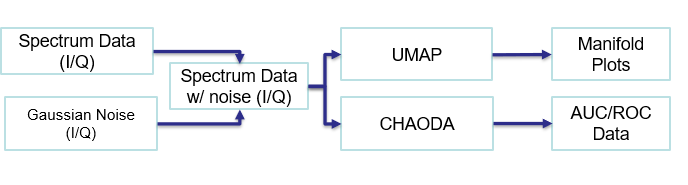
\includegraphics[width = 8cm]{Capture.png}
\caption{Model of Data Analysis}
\label{model}
\end{figure}

\section{Methods}
\subsection{RadioML Dataset}
The RadioML 2018 HDF5 dataset available from DeepSig \cite{b9} was selected to support my analysis as it has already been validated and highly leveraged for research in machine learning signal classification experiments which would provide benefits for comparative analysis in performance.  RadioML 2018 contains both live over the air and synthetically generated signal captures of different modulation modes over a range of SNR levels.  Specifically, the data is comprised of 24 modulation modes at SNR levels ranging from -20 dB to 30 dB in increments of 2 dB or 26 levels. Each modulation + SNR level has 4,096 samples. Therefore, the complete data set contains 2,555,504 (24 x 26 x 4,096) samples.  Each sample is comprised of a window of 1,024 points of In-phase and Quadrature 32-bit floating-point numbers stored as a single element in a the ‘X’ dataset. The ‘Y’ dataset correlates to each sample and is a 24-element array of modulation mode labels represented in a binary series with 1 identifying the modulation mode for that sample and lastly a third dataset ‘Z’ with a single value of the SNR provided for each sample. Therefore, each sample provided in RadioML 2018 can be thought of as a high dimensional array of 2048 floating point features for a single signal capture with labels for SNR as well as modulation mode. 

Modulation modes excite different signal manifestations as they each have historically different purposes and use cases. Table ~\ref{RadioML Modulation Modes} provides a summary of all of the modulation modes contained within the RadioML 2018 dataset. In Figures ~\ref{Sample Constellation Plots OOK to 8PSK},~\ref{Sample Const Plots 16PSK to 128APSK},~\ref{Sample Const Plots 16QAM to AM-SSB-WC},~\ref{Sample Const Plots AM-SSB-SC to OQPSK} I have provided constellation diagrams for samples generated from the I/Q data over time at 30 dB, 0 dB and -20 dB. They help depict the ease to complexity with relation to the structure of the individual data vector once the SNR drops. Figure ~\ref{Sample Plots IQ captures} provides some sample plots at 30 dB of each of the modulation modes from these we can see how the modulation modes exhibit different wave forms. Lastly, Figure ~\ref{Sample Plots IQ captures converted to magnitude} converts the I/Q to magnitude using the formula $Magnitude = \sqrt{I^{2}+Q^{2}}$ which is a better representation of the original power captured from in the sample.

\begin{table}
\centering
\caption{RadioML 2018 Modulation Modes}
\begin{tabular}{|l|l|l|} 
\hline
\multicolumn{1}{|c|}{\begin{tabular}[c]{@{}c@{}}\textbf{Modulation}\end{tabular}} & \multicolumn{1}{c|}{\textbf{Description}} & \multicolumn{1}{c|}{\textbf{Typical Use}}\\ 
\hline OOK 
& \begin{tabular}[c]{@{}l@{}}On-Off Keying\end{tabular} 
& \begin{tabular}[c]{@{}l@{}} Morse Code\end{tabular}\\ 
\hline 4ASK 
& \begin{tabular}[c]{@{}l@{}}Quaternary Amplitude\\Shift Keying\end{tabular} 
& \begin{tabular}[c]{@{}l@{}}Low-Frequency RF, \\Home automation devices, \\Tire Pressure Monitoring\end{tabular}\\ 
\hline 8ASK                                                                                             
& \begin{tabular}[c]{@{}l@{}}Quaternary Amplitude\\~Shift Keying\end{tabular}                         
& \begin{tabular}[c]{@{}l@{}}Low-Frequency RF, \\Home automation devices, \\Tire Pressure Monitoring\end{tabular}\\ 
\hline BPSK                                                                                             
& \begin{tabular}[c]{@{}l@{}}Binary Phase\\~Keying\end{tabular}                                                                                  
& \begin{tabular}[c]{@{}l@{}}Wireless communications,\\CDMA, Satellite, DVB, \\Cable Modems\end{tabular}\\ 
\hline QPSK                                                                                             
& \begin{tabular}[c]{@{}l@{}}Quadrature Phase\\~Shift Keying\end{tabular}                             
& \begin{tabular}[c]{@{}l@{}}Satellite Communications,\\MPEG2 Video, \\Cable Modems, \\Mobile phones\end{tabular}\\ 
\hline 16PSK                                                                                            
& \begin{tabular}[c]{@{}l@{}}16 Phase Shift Keying\end{tabular}                                                                                                                                                     
& \begin{tabular}[c]{@{}l@{}}Wireless LANs, RFID\end{tabular}\\ 
\hline 32PSK                                                                                            
& \begin{tabular}[c]{@{}l@{}}32 Phase Shift Keying\end{tabular}                                                                                                                                                                 
& \begin{tabular}[c]{@{}l@{}}Wireless LANs, RFID\end{tabular}\\
\hline 16APSK                                                                                           
& \begin{tabular}[c]{@{}l@{}}16 Phase - Amplitude \\and Phase Shift Keying\end{tabular}               
& \begin{tabular}[c]{@{}l@{}}Satellite Communications\end{tabular}\\ 
\hline 32APSK                                                                                           
& \begin{tabular}[c]{@{}l@{}}32 Phase - Amplitude\\and Phase Shift Keying\end{tabular}                
& \begin{tabular}[c]{@{}l@{}}Satellite Communications\end{tabular}\\ 
\hline 64APSK                                                                                           
& \begin{tabular}[c]{@{}l@{}}64 Phase - Amplitude\\and Phase Shift Keying\end{tabular}                
& \begin{tabular}[c]{@{}l@{}}Satellite Communications\end{tabular}\\ 
\hline 128APSK                                                                                          
& \begin{tabular}[c]{@{}l@{}}128 Phase - Amplitude \\and Phase Shift Keying\end{tabular}              
& \begin{tabular}[c]{@{}l@{}}Satellite Communications\end{tabular}\\ 
\hline 16QAM                                                                                            
& \begin{tabular}[c]{@{}l@{}}16 State - Quadrature\\Amplitude Modulation\end{tabular}                 
& \begin{tabular}[c]{@{}l@{}}Higher Data Rates, \\Digital Terrestrial \\Television\end{tabular}\\ 
\hline 32QAM                                                                                            
& \begin{tabular}[c]{@{}l@{}}32 State- Quadrature\\Amplitude Modulation\end{tabular}                  
& \begin{tabular}[c]{@{}l@{}}Higher Data Rates\end{tabular}\\  
\hline 64QAM                                                                                            
& \begin{tabular}[c]{@{}l@{}}64 State- Quadrature\\Amplitude Modulation\end{tabular}                  
& \begin{tabular}[c]{@{}l@{}}Higher Data Rates, \\Digital Cable,\\Digital Terrestrial \\Television\end{tabular}\\ 
\hline 128QAM                                                                                           
& \begin{tabular}[c]{@{}l@{}}128 State- Quadrature\\Amplitude Modulation\end{tabular}                 
& \begin{tabular}[c]{@{}l@{}}Higher Data Rates\end{tabular}\\ 
\hline 256QAM                                                                                           
& \begin{tabular}[c]{@{}l@{}}256 State- Quadrature \\Amplitude~Modulation\end{tabular}                
& \begin{tabular}[c]{@{}l@{}}Higher Data Rates, \\Digital Cable\end{tabular}\\ 
\hline AM-SSB-WC                                                                                        
& \begin{tabular}[c]{@{}l@{}}Amplitude Modulation \\Single Sideband \\With Carrier\end{tabular}       
& \begin{tabular}[c]{@{}l@{}}Air, Land \& Maritime \\Communications\end{tabular}\\ 
\hline AM-SSB-SC                                                                                        
& \begin{tabular}[c]{@{}l@{}}Amplitude Modulation\\Single Sideband \\Supressed Carrier\end{tabular}   
& \begin{tabular}[c]{@{}l@{}}Analog Television \\Broadcast,\\Radio Data Systems\end{tabular}\\ 
\hline AM-DSB-WC                                                                                        
& \begin{tabular}[c]{@{}l@{}}Amplitude Modulation \\Double Sideband \\With Carrier\end{tabular}       
& \begin{tabular}[c]{@{}l@{}}Broadcast Radio, \\Aircraft Communications\end{tabular}\\ 
\hline AM-DSB-SC                                                                                        
& \begin{tabular}[c]{@{}l@{}}Amplitude Modulation\\Double Sideband \\Suppressed Carrier\end{tabular} 
& \begin{tabular}[c]{@{}l@{}}Radio Data Systems\end{tabular}\\ 
\hline FM  
& \begin{tabular}[c]{@{}l@{}}Frequency Modulation\end{tabular} 
& \begin{tabular}[c]{@{}l@{}}FM Radio, telemetry, Radar\end{tabular}\\ 
\hline GMSK                                                                                             
& \begin{tabular}[c]{@{}l@{}}Gaussian Minimum\\Shift Keying\end{tabular}                             
& \begin{tabular}[c]{@{}l@{}}High Data Rates, \\Bluetooth, \\Satellite Communications\end{tabular}\\ 
\hline OQPSK                                                                                            
& \begin{tabular}[c]{@{}l@{}}Offset Quadrature \\Phase Shift Keying\end{tabular}                      
& \begin{tabular}[c]{@{}l@{}}Mobile Radio Systems, \\Home Automation\end{tabular}\\
\hline
\end{tabular}
\label{RadioML Modulation Modes}
\end{table}

\subsection{Dividing the Dataset}
In an effort to better determine channel availability I decomposed the dataset in to new H5 files for each modulation mode thus allowing me to conduct exploration of a UMAPs and conducting test runs against CHAODA more easily. The approach of dividing the dataset also allowed for targeted analysis of various modulation modes with relative ease and the production of scenarios that would aid in future exploration.

\subsection{Adding Noise}
All the data captured in the RadioML 2018 dataset contain a signal with varying levels of SNR.  The dataset in its provisioned condition would not allow for determining channel availability only signal detection. Consider the condition where a perfect detection system could be developed, all the entries in RadioML 2018 would be found to be a signal with no instances of noise without a signal. Since our goal is to determine noise or signal, we need to correct this by adding noise. A method of noise generation was created through the use of GNURadio \cite{b8} which is a python/C++ object based development environment supporting software defined radios.  I/Q data was collected by leveraging the blocks illustrated in Figure ~\ref{GNURADIO}. The noise I/Q samples were then merged with the RadioML dataset and a label with a modulation mode of “Noise” and the SNR label of -50  dB was applied although no signal is present so there is no measurable level. Noise is then applied to each individual set of modulation samples at a $9:1$ ratio. Since each Modulation mode and SNR combination is 4,096 samples we add 36,864 samples of Gaussian noise allowing for the signal to now become an outlier or anomaly making up 10\% of the samples analyzed.

\begin{figure}
\centering
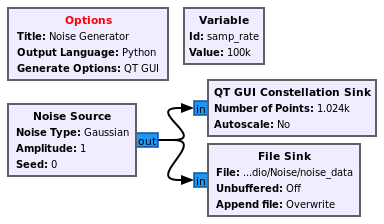
\includegraphics[width = 8cm]{GNURADIO_NOISE_2.png}
\caption{GNU Radio Noise Generation Blocks}
\label{GNURADIO}
\end{figure}

\subsection{Exploring RadioML with UMAP}
Leveraging the UMAP method we then attempt to evaluate the entire RadioML dataset to reveal a global structure that perhaps could give an understanding of clustering performance.  If the structure indicates clear separation between higher SNR values and lower values then it could be assumed that the capability of a clustering algorithm to discover related structures may not be possible should data be more integrated it may illustrate that the data itself may be correlated however as the dataset is not integrated with noise this may not be beneficial as the relation to pure noise is not evident. 

\subsection{Clustering Hierarchical methods for signal detection}
CHAODA provides an outlier detection approach that is built on Clustered Learning of Approximate Manifolds (CLAM) by applying an ensemble of methods to analyze the resulting graph.  CLAM and sequentially CHAODA work well on datasets that have high-dimensions by mapping them to a lower dimensional graph that represent an approximate manifold of the original data.  CHAODA currently uses six methods in its ensemble, cluster cardinality, parent cardinality, component cardinality, vertex degree, graph neighborhood and stationary probabilities.  The results from each of these methods is then averaged and provided as a measure against the Reciever Operating Characteristic (ROC) and is presented as Area Under the ROC Curve (AUC). In support of this investigation the modified RadioML 2018 data with additive noise will have CHAODA applied and a AUC measure will be collected against each modulation mode at each incremental 2 dB SNR level provided.  I will then examine the results and determine how CHAODA performs as a signal detector by treating noise as the inlier and the signal as an outlier.  

\subsection{Supporting Test materials}
In support of my test methods I leveraged a Dell PowerEdge T630 server with two intel Xeon E5-2697 v3 processors hosting 14 cores (28 threads) thus supporting a total of 56 threads.  The system has 220GB of RAM, a 1TB Solid state drive 4TB hard disk drive and a NVIDA 980 ti GPU with 6GB video ram.  Testing was conducted using Ubuntu 20.04 server operating system, Python 3.8 with a large list of supporting packages for UMAP and CHAODA.

\section{Results}
\subsection{Reviewing global and local structure using UMAP}
Attempts to process the entire dataset via UMAP lead to repeated kill commands being issued by the python environment. Researching this a bit discovered that was an underlying bug in numba python package that is know to cause crashes with large datasets. Only randomly selected 40\% of the dataset could be successfully processed by UMAP.  The global structure is revealed in Figure ~\ref{UMAP_40A}.  In this we can clearly see that the noise datapoints are not as integrated as we hoped for signals below -10dB there does appear to be opportunities in the signals 30dB to -10dB to further explore each of the modulation modes independently evaluated them in UMAP separately and were able to conduct a compete evaluation on each of them as shown in Figure.  A separate evaluation of the noise was conducted as depicted in Figure~\ref{noise}.  As we see the structure for the Gaussian noise is structurally similar as expected and should serve as a good basis for comparison against those values that have low SNR values.

\subsection{Analysis of UMAP presentation of RadioML}
Fig.~\ref{UMAP Plots} contains plots for all of the UMAP models associated with every modulation mode provided in the RadioML 2018 dataset and are represented without pure noise added.  OOK and ASK plots indicate clear separation between the high and low SNR signals indicating separation of the data lending itself for effective outlier detection. PSK and QAM modulation modes starting with BPSK to 256QAM all have similar presentations with the high and low level SNR values being clustering together indicating the potential for separability and classification.  The remaining modes starting at AM-SSC-WC and ending with OQPSK all appear have very different and unique representations which still provide separation however there are very little instances of the mid to low value SNR levels being grouped across a transition space which may tell us that our data isn't going to be effective in those area. 

Fig.~\ref{UMAP Noise Plots} are UMAP plots of the same data provided in Fig.~\ref{UMAP Plots} however this time with a ration of $9:1$ noise.  Plots of these were created to allow for some insight into the manifold of noise in contract to the proposed outliers or signal provided by RadioML.  Examining these UMAP plots we see that in almost all of them there is a distinction between high SNR values and noise.  Unfortunately the view also shows us that the mid to low value scores tend to be generalized with the noise this will have to be examined further to determine how they can better be associated with higher SNR results thus providing better detection.

\subsection{Signals as outliers evaluated with CHAODA}
Evaluation across the entire RadioML 2018 dataset with additive noise took approximately 97 hours to complete.  Fig.~\ref{Part1_results} provides results for modulation modes OOK to  128APSK this was done to provide plots that could be more easily reviewed. Results for OOK, 4ASK and 8ASK were very promising as they indicate a clear determination of signal recognition starting at -8 dB with results almost near perfect  by the time SNR reaches -4 dB.  The remainder of the PSK modes though have varying results but appear to provide Area Under the ROC Curve (AUC) scores with measurable improvement by 4 dB.  Reviewing Fig.~\ref{Part2_results} we examine the QAM and AM modulation modes we again see immediately postive results starting as low as -8 dB for 16QAM and AM-SSB-WC and the majority of the modulation modes show some signs of detection as an outlier after 2 dB.   Captured in Table ~\ref{CHAODA AUC Scores -20 to 0} are the AUC scores for test runs representing data in the more noise intensive environments these would be the more challenging results.  Table ~\ref{CHAODA AUC Scores 2 to 30} encompasses the AUC scores for environments where the signal is predominate over noise and there for should be easily identified.  Results were also examined for performance at various noise levels for BPSK, in Fig.~\ref{Part3_results} we see that adding noise does not seem to improve results whereas removing noise seems to create less success at detection likely due to the less generalization of noise provided by fewer samples added as inliers. 

\begin{figure}[htbp]
\centering
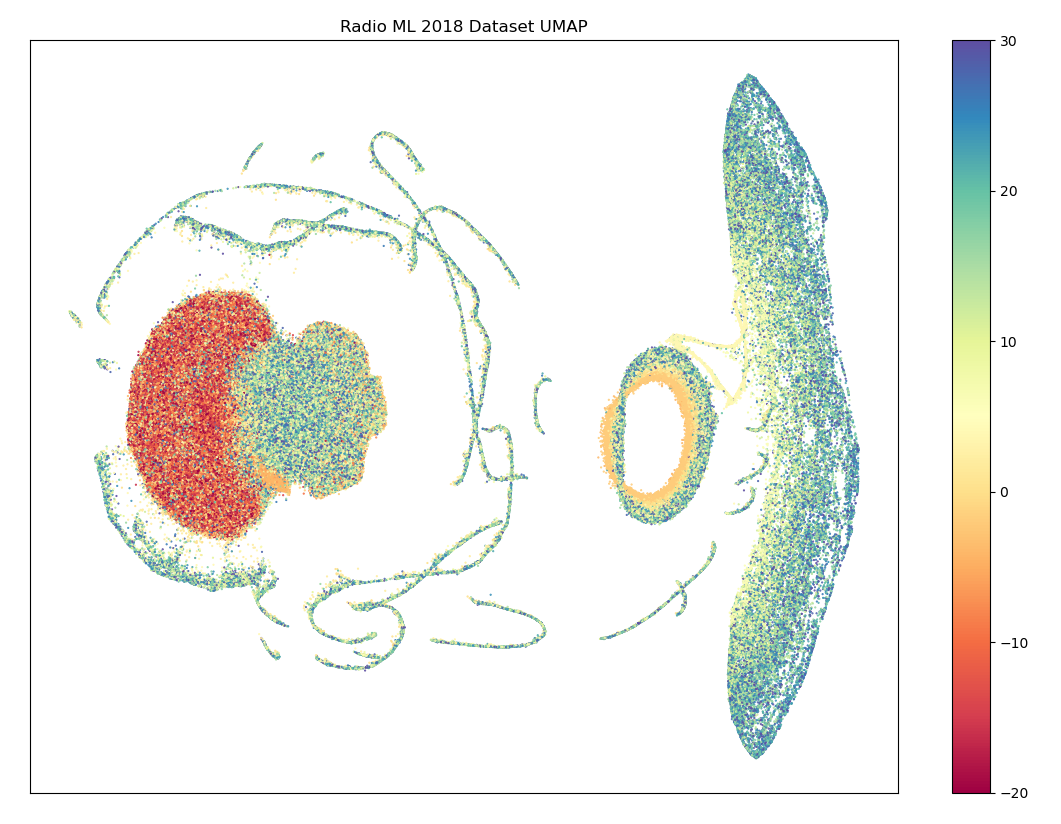
\includegraphics[width = 8cm]{/UMAP/Figure_211008_40A.png}
\caption{UMAP plot of the RadioML dataset(40\%)}
\label{UMAP_40A}
\end{figure}

\begin{figure}[htbp]
\centering
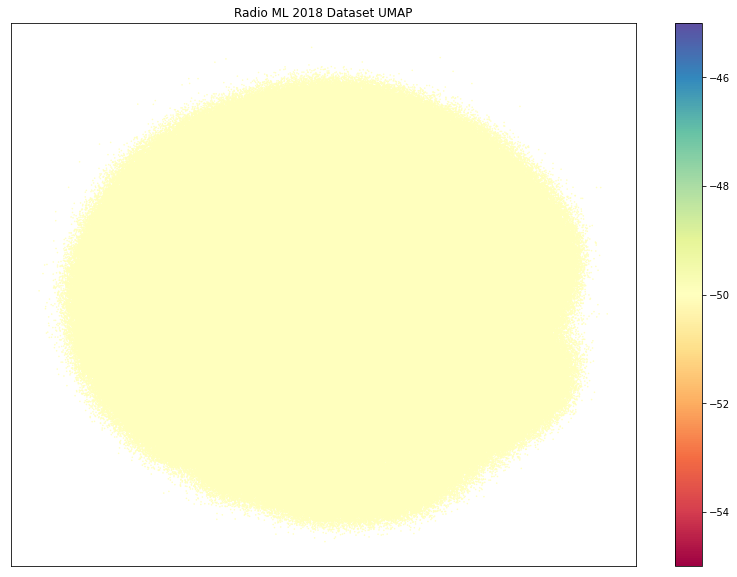
\includegraphics[width = 8cm]{/UMAP/Figure 2021-11-26 190618.png}
\caption{UMAP plot of Generated Noise}
\label{noise}
\end{figure}

\begin{figure}[htbp]
\centering
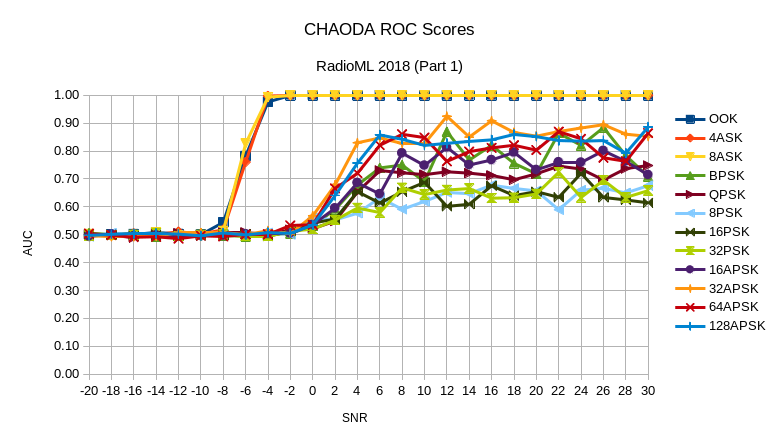
\includegraphics[width = 8.8cm]{/Results/Part1_AUC.png}
\caption{Part 1 - CHAODA AUC Scores (OOK - 128APSK)}
\label{Part1_results}
\end{figure}

\begin{figure}[htbp]
\centering
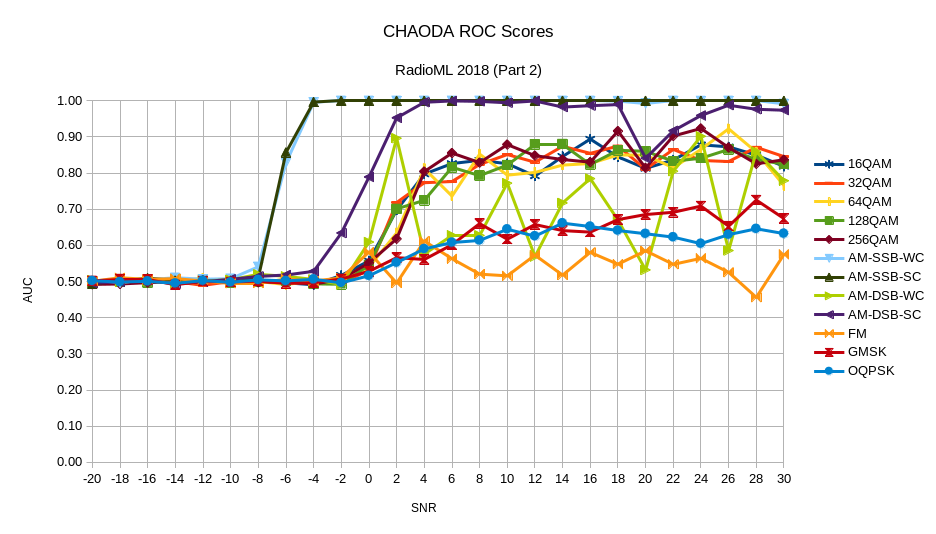
\includegraphics[width = 8.8cm]{/Results/Part2_AUC_corrected.png}
\caption{Part 2 - CHAODA AUC Scores (16QAM - OQPSK)}
\label{Part2_results}
\end{figure}

\begin{figure}[htbp]
\centering
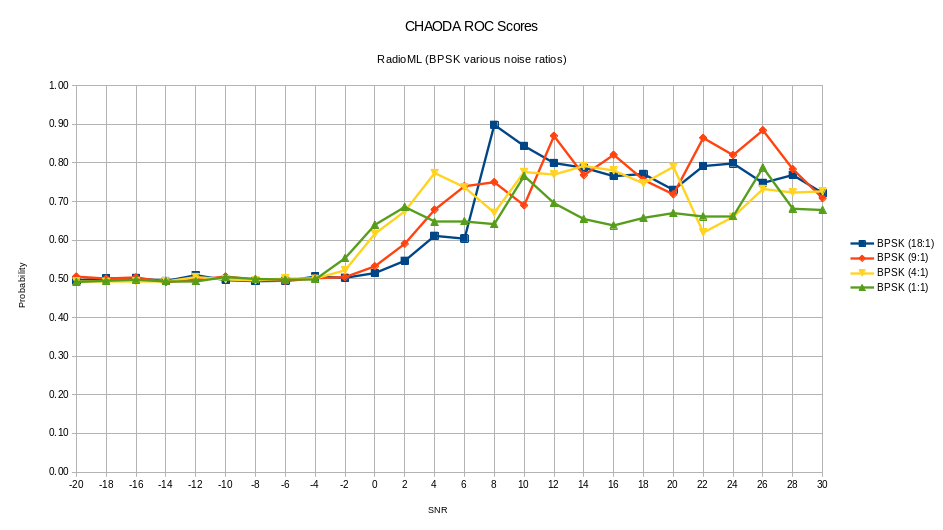
\includegraphics[width = 8.8cm]{/Results/Part3_noise.png}
\caption{Varying Noise CHAODA AUC Scores (BPSK)}
\label{Part3_results}
\end{figure}

\section{Conclusion and Future Work}
\subsection{Significant Issues}
During the testing and evaluation of RadioML it was uncovered that the incorrect sequence of modulation modes was provided in the "classes.txt" file within the compressed RadioML 2018 dataset. As a result, the labels specifically provided for the ‘Y’ dataset were not correct. While this did not significantly impact the evaluation of the data it did allow for ineffective correlation to previous results as well as impact any results built from the parsing of the dataset into modulation mode segments for evaluation. The accurate order of the classes (modulation modes) however was provided in the supporting paper "Over-the-Air Deep Learning Based Radio Signal Classification,"  under Fig. 12. and was also discussed on an independent reviewers website, 'DeepSig’s 2018 Data Set: 2018.01.OSC.0001\_1024x2M. h5.tar.gz' where a more in depth assessment is provided. 

\subsection{Conclusions}
The effort of performing outlier detection using the modified RadioML 2018 dataset confirmed that CHAODA’s transfer learning approach is effective as no training was required and the entire effort was unsupervised. CHAODA's approach yielded some signal detection starting at 0 dB.  It should be also noted that the information that the system had been previously trained upon did not have a feature set that corresponded to anything similar to RadioML 2018 which is a strong avocation that CHAODA can be leveraged as an unsupervised method on new data without modification.

Secondly, the development of a characteristic noise manifold can allow for effective outlier detection of signals and that quite possibly with an additional distance metric and perhaps retraining of the CHAODA meta-models further improvements may be possible. Increasing the ratio of the noise beyond the $9:1$ ratio used during the test may not provide any benefit however utilizing less noise does tend to reduce AUC scores. Additional testing should be conducted to better generalize the appropriate manifold for noise.

Lastly after some review, the dataset seems to be triggering a detection largely where amplitude is involved and less so when the modulation method is frequency based.  Intuition is that amplitude data presents itself more clearly as a structure change with rising and falling values however frequency is captured in the period or occurrence data therefore perhaps the feature set itself would benefit from being appended by a Fast Fourier Transform (FFT) over the points and better capture shifts in frequency.

\subsection{Future Efforts}
In future efforts I will examine the “New Approaches of Automatic Modulation Classification based on in Phase-Quadrature Diagram Combined with Artificial Neural Network” \cite{b12} and determine if any of the approaches outlined could be added or adapted to the CHAODA ensembles methods and improve results. In addition, the Multistage Clustering based Automatic Modulation Classification also holds some opportunity at tackling this if the CHAODA methods could tackle multiclass outlier identification \cite{b13}.  

\begin{thebibliography}{00}
\bibitem{b1}United States, Federal Communications Commission. "Facilitating Opportunities for Flexible, Efficient and Reliable Spectrum Use Employing Cognitive Radio Technologies." 69 FR 7397-7411 (02/17/2004)
\bibitem{b2}Saleem, Yasir, Mubashir Husain Rehmani, and Sherali Zeadally. "Integration of cognitive radio technology with unmanned aerial vehicles: issues, opportunities, and future research challenges." Journal of Network and Computer Applications 50 (2015): 15-31
\bibitem{b3}Reyes, Hector, Nickolas Gellerman, and Naima Kaabouch. "A cognitive radio system for improving the reliability and security of UAS/UAV networks." 2015 IEEE Aerospace Conference. IEEE, 2015.
\bibitem{b4}Cacciapuoti, Angela Sara, et al. "Channel availability for mobile cognitive radio networks." Journal of Network and Computer Applications 47 (2015): 131-136.
\bibitem{b5}R. Tandra and A. Sahai, "SNR Walls for Signal Detection," in IEEE Journal of Selected Topics in Signal Processing, vol. 2, no. 1, pp. 4-17, Feb. 2008, doi: 10.1109/JSTSP.2007.914879.
\bibitem{b6}M. A. Hammouda and J. W. Wallace, "Noise uncertainty in cognitive radio sensing: Analytical modeling and detection performance," 2012 International ITG Workshop on Smart Antennas (WSA), 2012, pp. 287-293, doi: 10.1109/WSA.2012.6181221.
\bibitem{b7}T. J. O’Shea, T. Roy and T. C. Clancy, "Over-the-Air Deep Learning Based Radio Signal Classification," in IEEE Journal of Selected Topics in Signal Processing, vol. 12, no. 1, pp. 168-179, Feb. 2018, doi: 10.1109/JSTSP.2018.2797022.
\bibitem{b8}“The Free \& Open-Source Radio Ecosystem · Gnu Radio.” GNU Radio, https://gnuradio.org
\bibitem{b9}Inc., DeepSig. “RF Datasets for Machine Learning.” \\DeepSig, https://www.deepsig.ai/datasets.
\bibitem{b10}McInnes, Leland, John Healy, and James Melville. "Umap: Uniform manifold approximation and projection for dimension reduction." arXiv preprint arXiv:1802.03426 (2018).
\bibitem{b11}Najjib Ishaq, Thomas Howard, and Noah Daniels. "Clustered Hierarchical Anomaly and Outlier Detection Algorithms," Nov. 2021
\bibitem{b12}Gouho, Jean Baptiste Bi, et al. "New approach of automatic modulation classification based on in phase-quadrature diagram combined with artificial neural network." International Journal of Advanced Computer Science and Applications 10.7 (2019): 141-145.
\bibitem{b13}Kalam, Lamia M., and Lakshmi N. Theagarajan. "Multistage clustering based automatic modulation classification." 2019 IEEE 89th Vehicular Technology Conference (VTC2019-Spring). IEEE, 2019
\end{thebibliography}
\vspace{12pt}

\onecolumn
\begin{figure*}
\centering
\subfloat{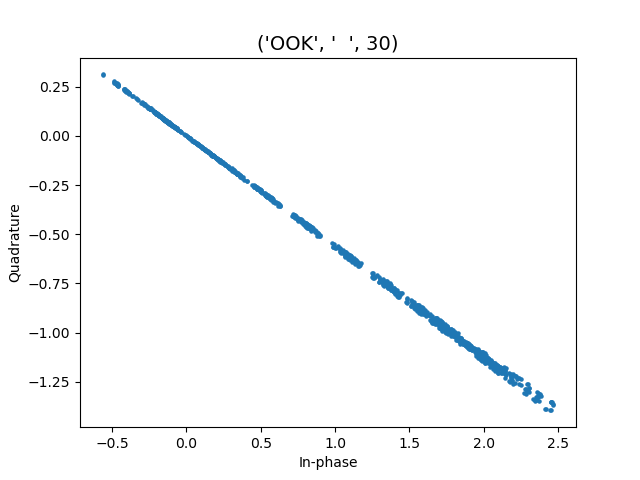
\includegraphics[width = 4.8cm]{/const/const_OOK_30.png}} 
\subfloat{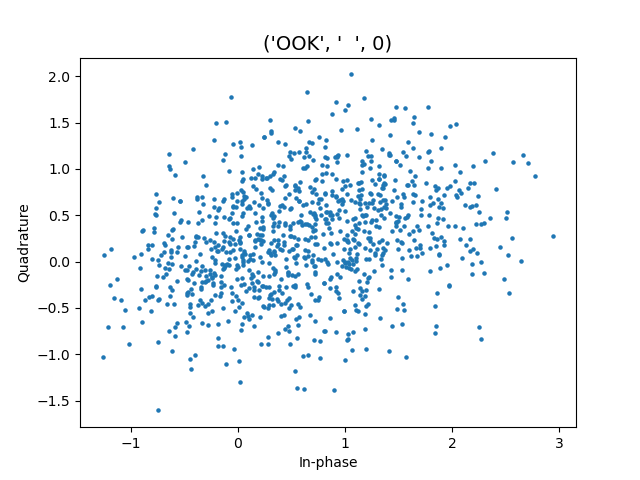
\includegraphics[width = 4.8cm]{/const/const_OOK_0.png}}
\subfloat{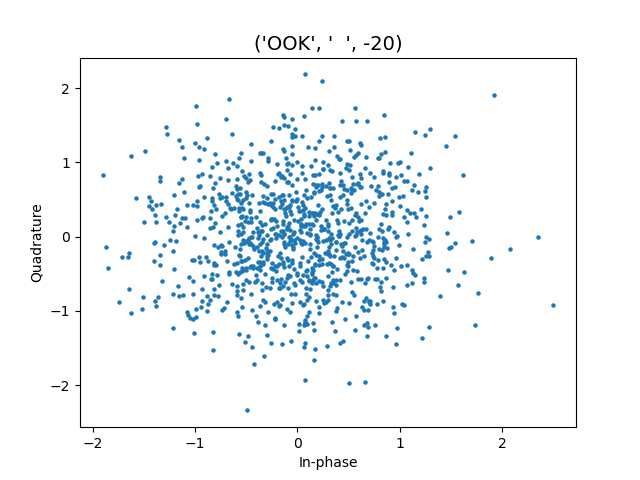
\includegraphics[width = 4.8cm]{/const/const_OOK_-20.png}}\\
\subfloat{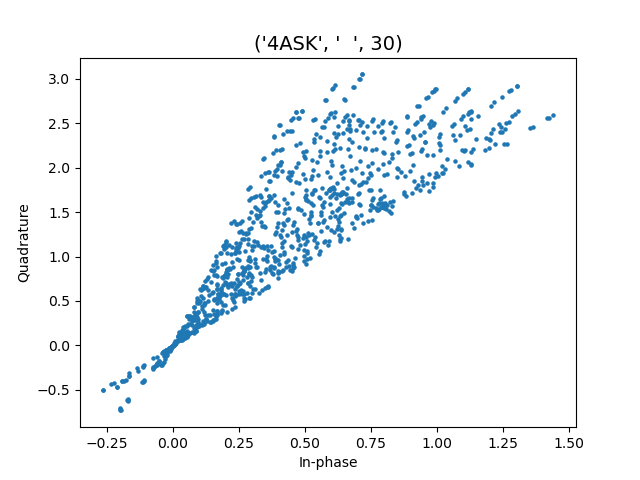
\includegraphics[width = 4.8cm]{/const/const_4ASK_30.png}} 
\subfloat{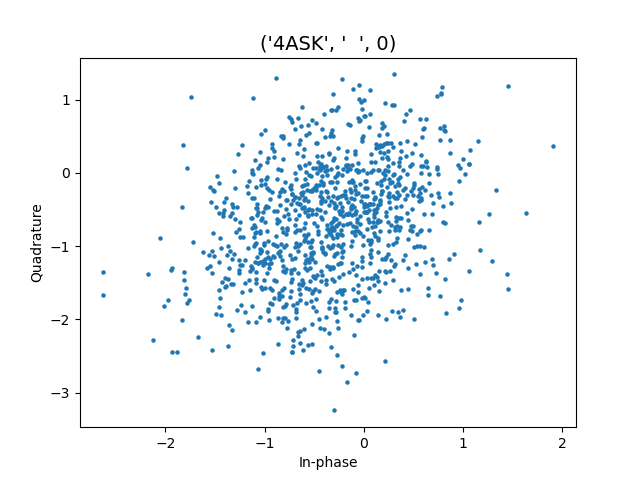
\includegraphics[width = 4.8cm]{/const/const_4ASK_0.png}}
\subfloat{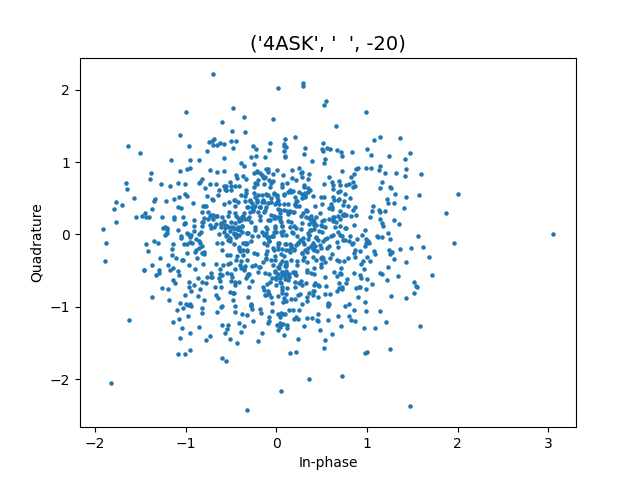
\includegraphics[width = 4.8cm]{/const/const_4ASK_-20.png}}\\
\subfloat{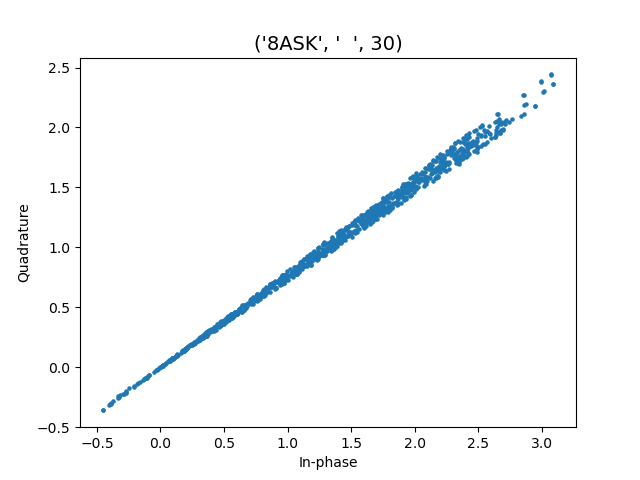
\includegraphics[width = 4.8cm]{/const/const_8ASK_30.png}} 
\subfloat{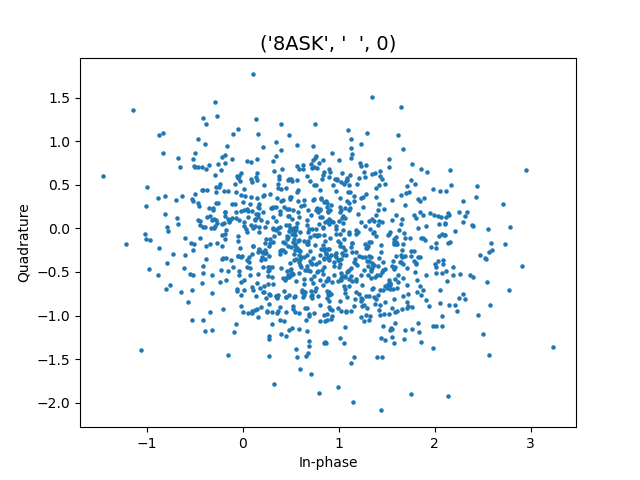
\includegraphics[width = 4.8cm]{/const/const_8ASK_0.png}}
\subfloat{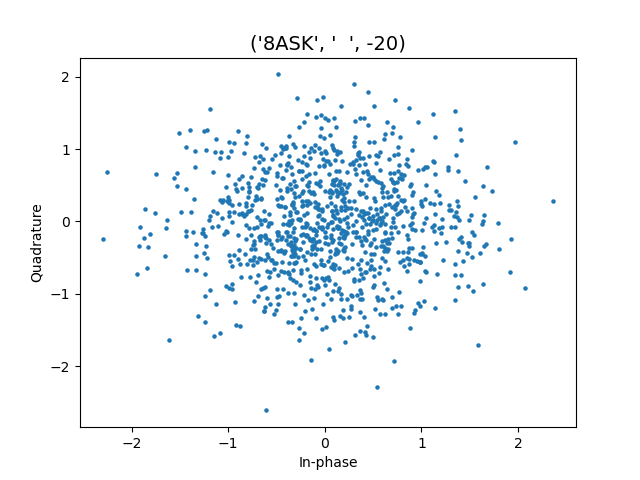
\includegraphics[width = 4.8cm]{/const/const_8ASK_-20.png}}\\
\subfloat{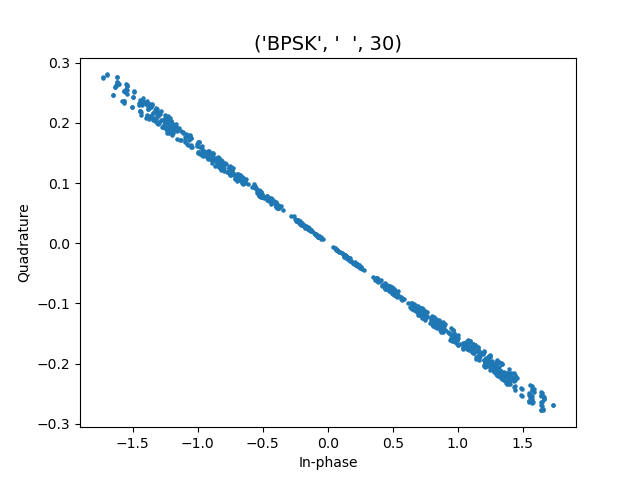
\includegraphics[width = 4.8cm]{/const/const_BPSK_30.png}} 
\subfloat{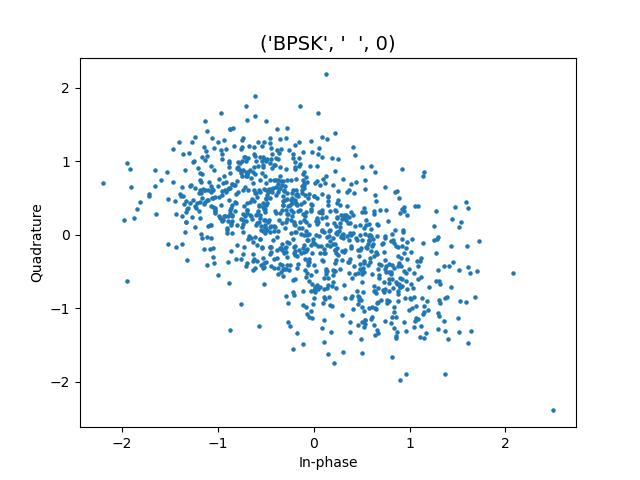
\includegraphics[width = 4.8cm]{/const/const_BPSK_0.png}}
\subfloat{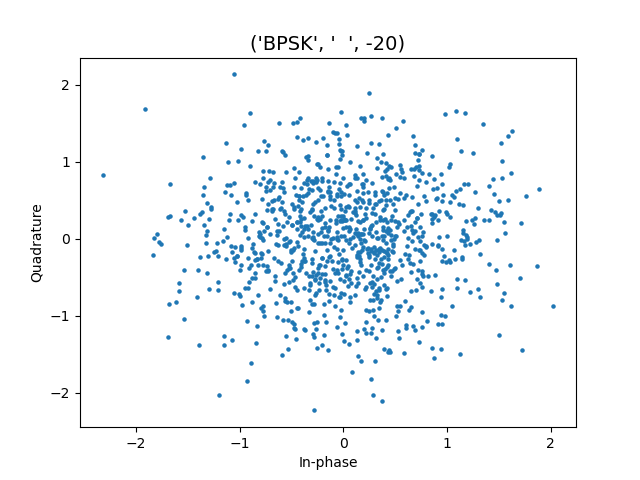
\includegraphics[width = 4.8cm]{/const/const_BPSK_-20.png}}\\
\subfloat{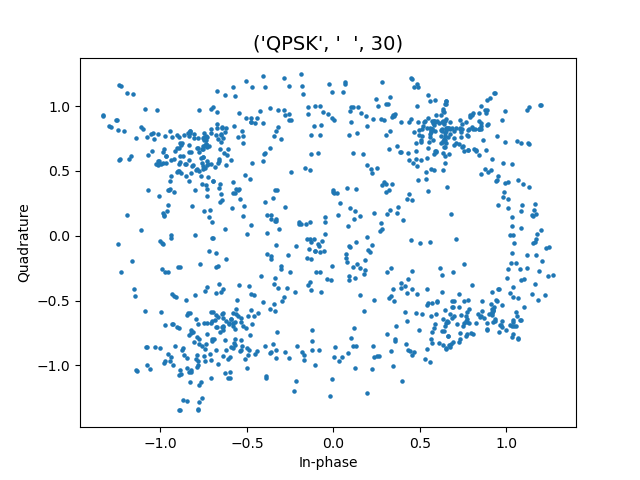
\includegraphics[width = 4.8cm]{/const/const_QPSK_30.png}} 
\subfloat{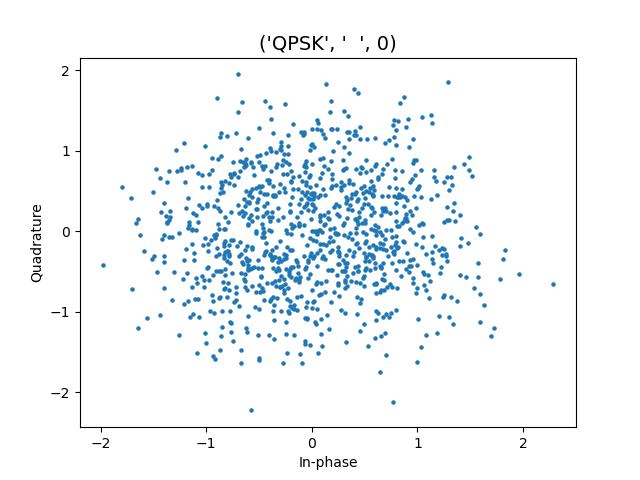
\includegraphics[width = 4.8cm]{/const/const_QPSK_0.png}}
\subfloat{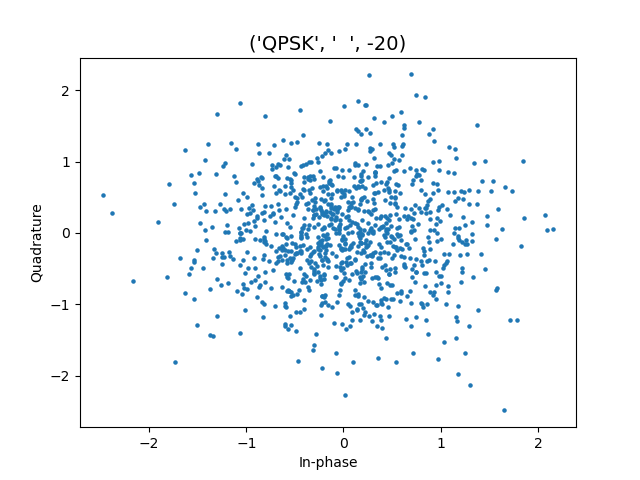
\includegraphics[width = 4.8cm]{/const/const_QPSK_-20.png}}\\
\subfloat{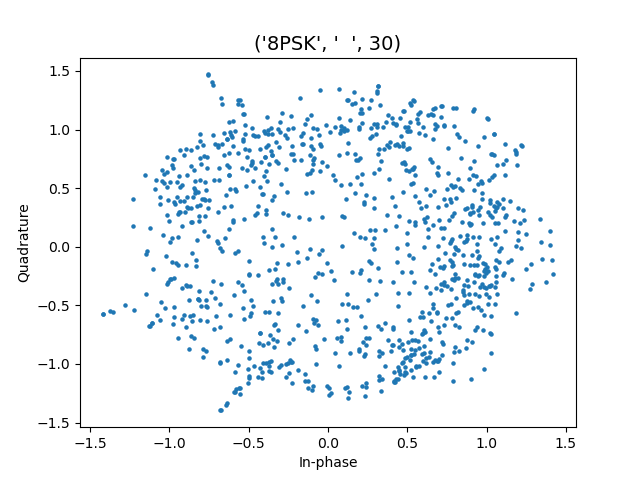
\includegraphics[width = 4.8cm]{/const/const_8PSK_30.png}} 
\subfloat{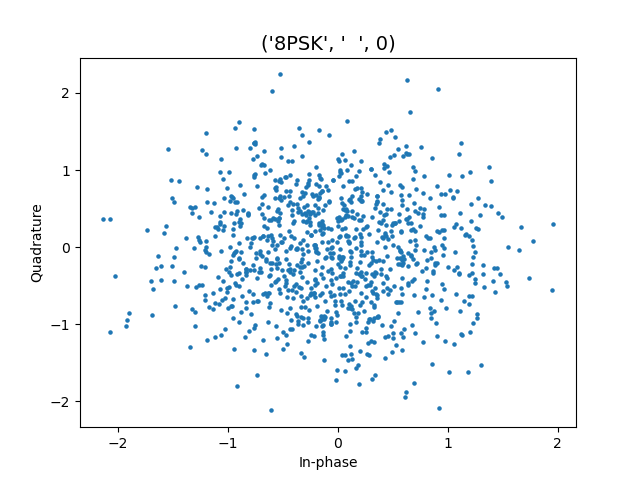
\includegraphics[width = 4.8cm]{/const/const_8PSK_0.png}}
\subfloat{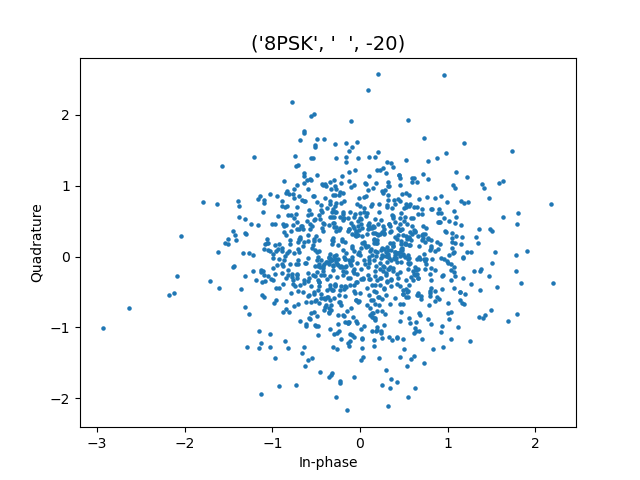
\includegraphics[width = 4.8cm]{/const/const_8PSK_-20.png}}\\
\caption{Sample Constellation Plots of Modulation modes OOK to 8PSK}
\label{Sample Constellation Plots OOK to 8PSK}
\vspace{-26pt}	 		
\end{figure*}

\begin{figure*}
\centering
\subfloat{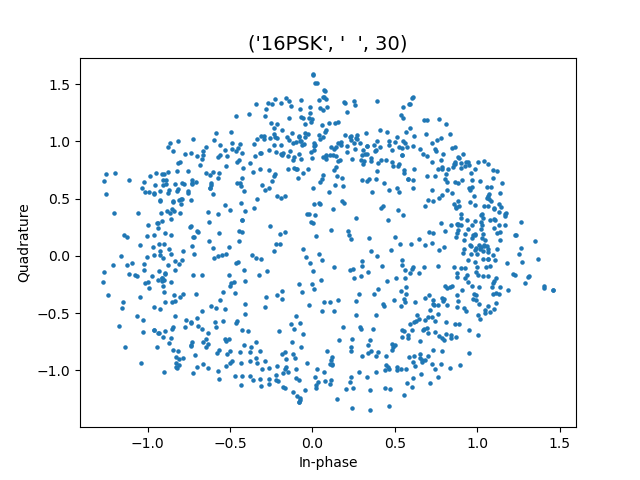
\includegraphics[width = 4.8cm]{/const/const_16PSK_30.png}} 
\subfloat{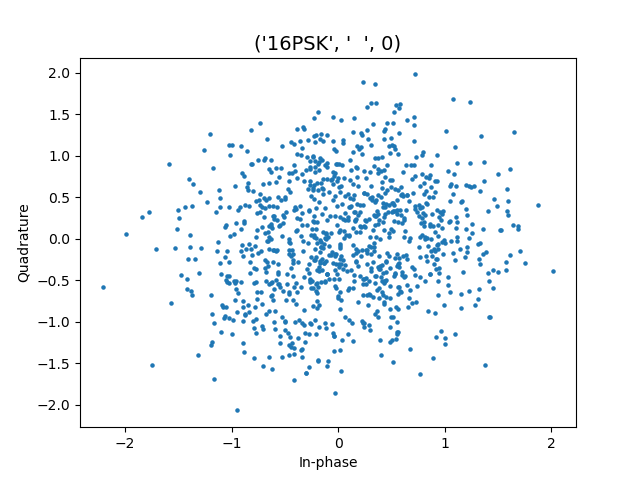
\includegraphics[width = 4.8cm]{/const/const_16PSK_0.png}}
\subfloat{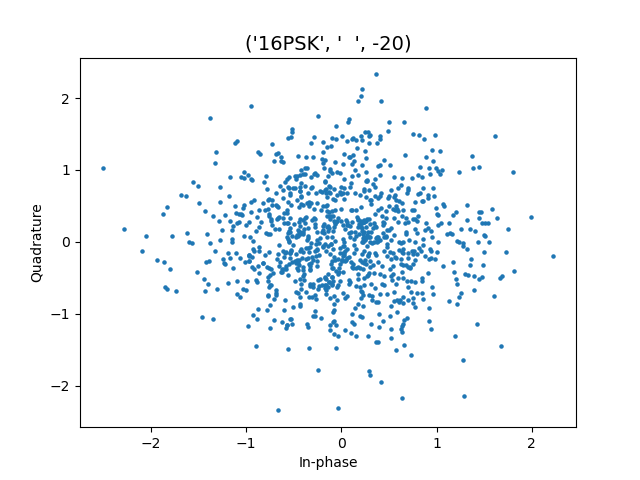
\includegraphics[width = 4.8cm]{/const/const_16PSK_-20.png}}\\
\subfloat{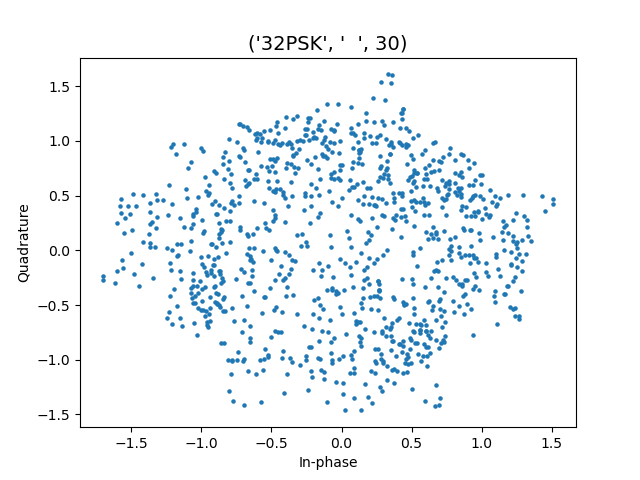
\includegraphics[width = 4.8cm]{/const/const_32PSK_30.png}} 
\subfloat{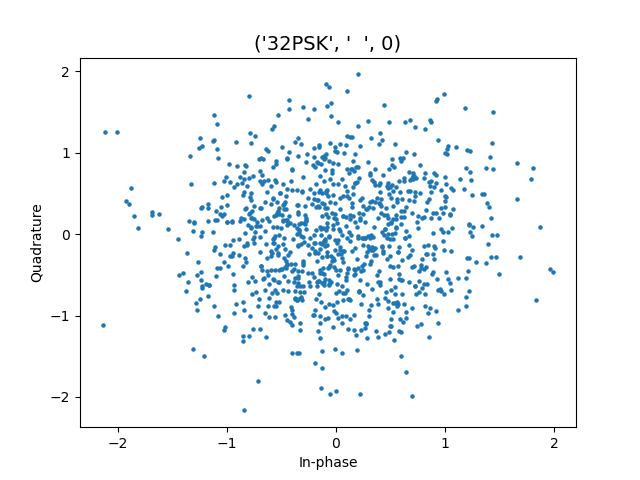
\includegraphics[width = 4.8cm]{/const/const_32PSK_0.png}}
\subfloat{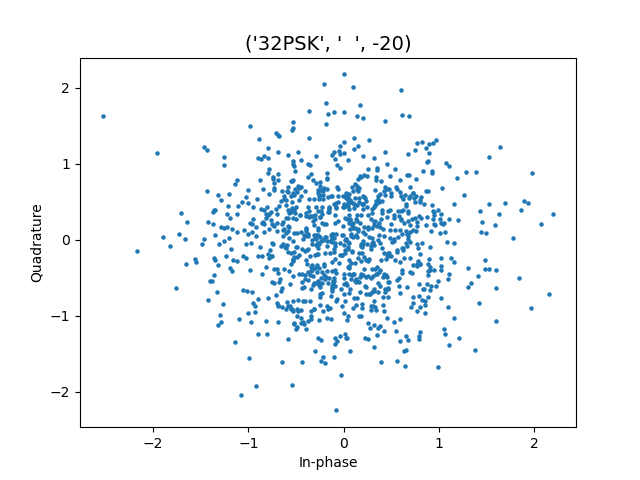
\includegraphics[width = 4.8cm]{/const/const_32PSK_-20.png}}\\
\subfloat{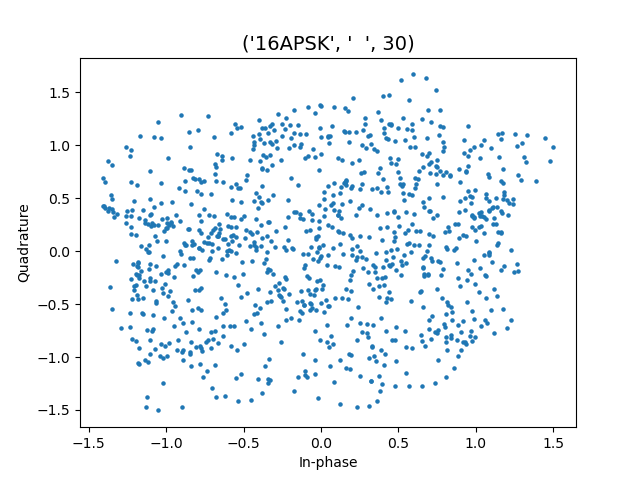
\includegraphics[width = 4.8cm]{/const/const_16APSK_30.png}} 
\subfloat{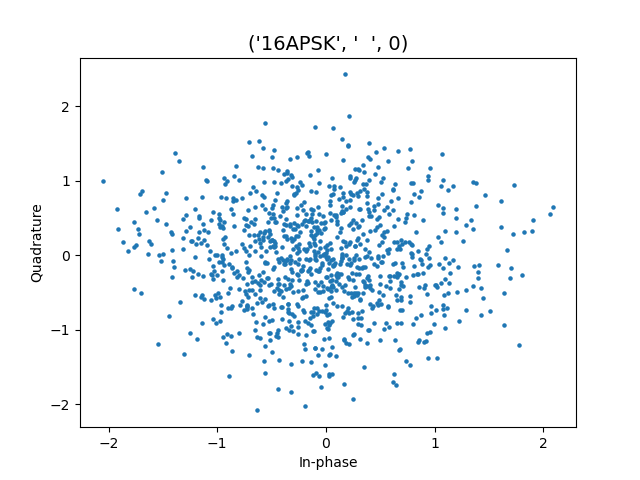
\includegraphics[width = 4.8cm]{/const/const_16APSK_0.png}}
\subfloat{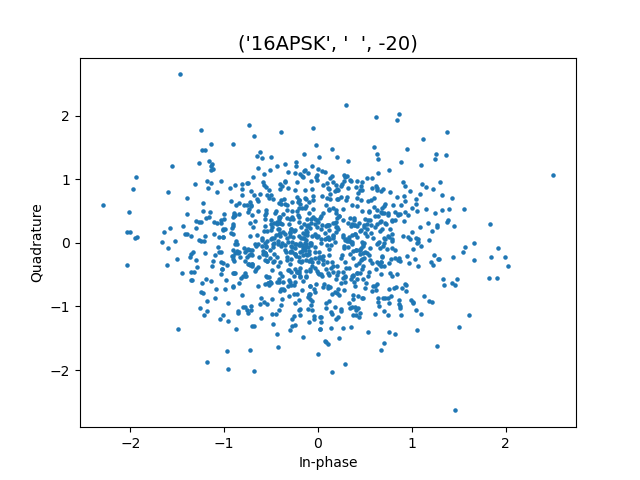
\includegraphics[width = 4.8cm]{/const/const_16APSK_-20.png}}\\
\subfloat{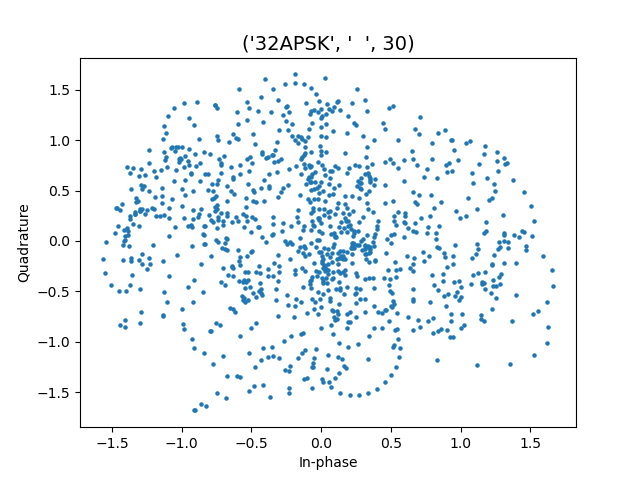
\includegraphics[width = 4.8cm]{/const/const_32APSK_30.png}} 
\subfloat{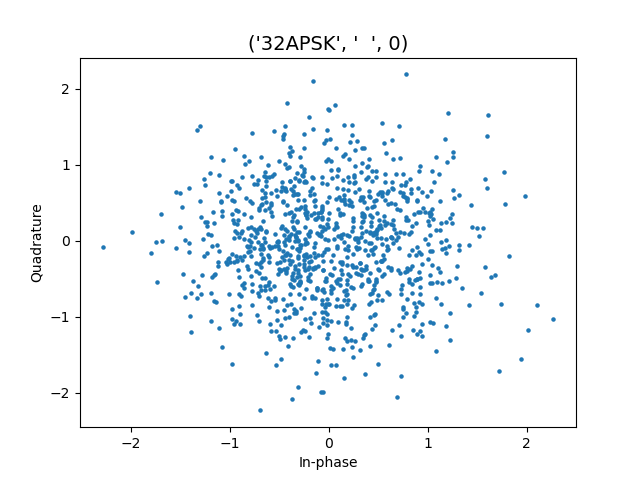
\includegraphics[width = 4.8cm]{/const/const_32APSK_0.png}}
\subfloat{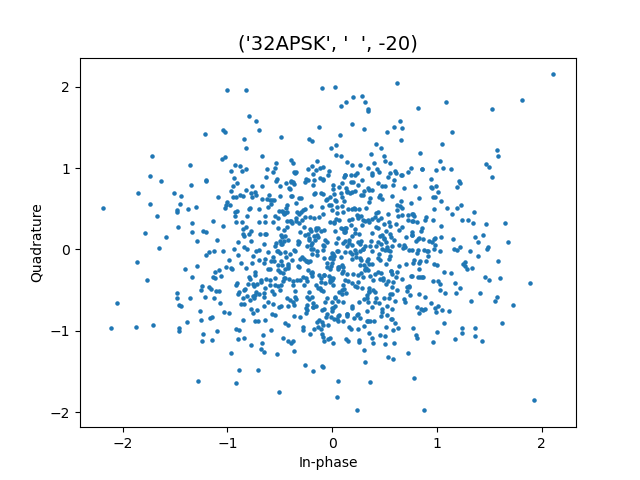
\includegraphics[width = 4.8cm]{/const/const_32APSK_-20.png}}\\
\subfloat{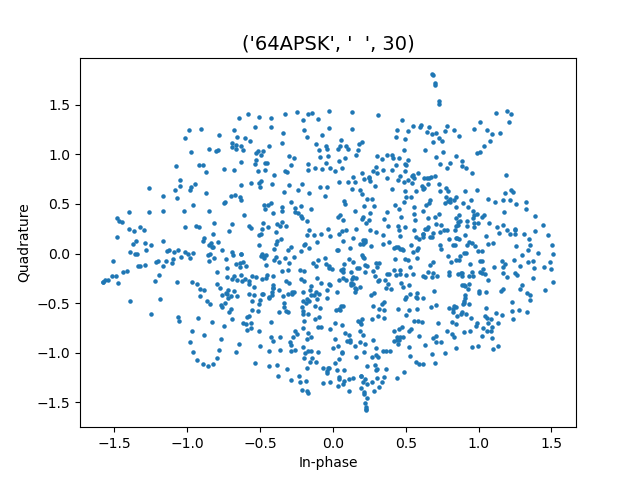
\includegraphics[width = 4.8cm]{/const/const_64APSK_30.png}} 
\subfloat{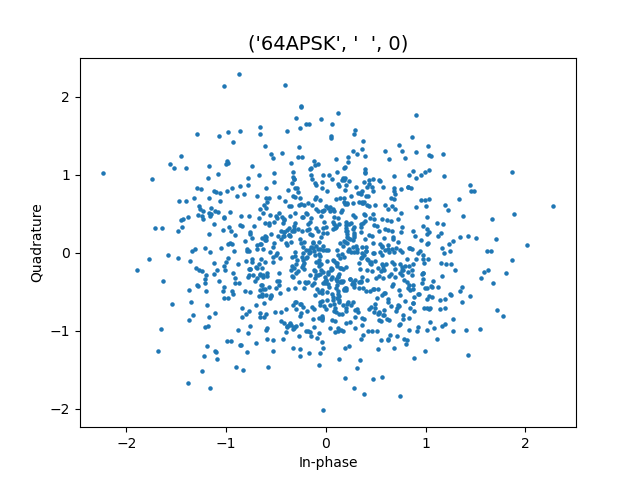
\includegraphics[width = 4.8cm]{/const/const_64APSK_0.png}}
\subfloat{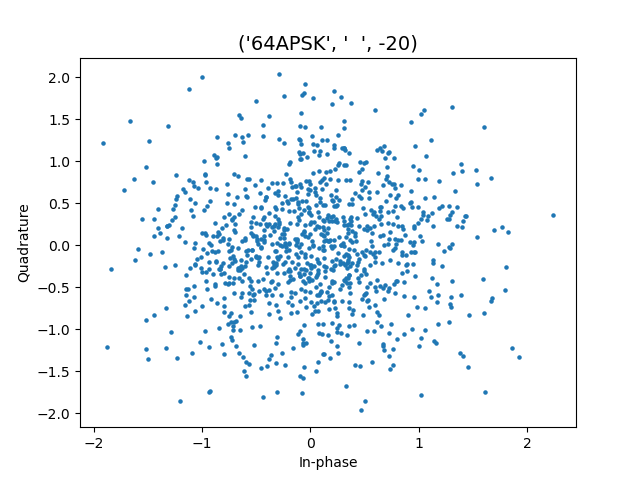
\includegraphics[width = 4.8cm]{/const/const_64APSK_-20.png}}\\
\subfloat{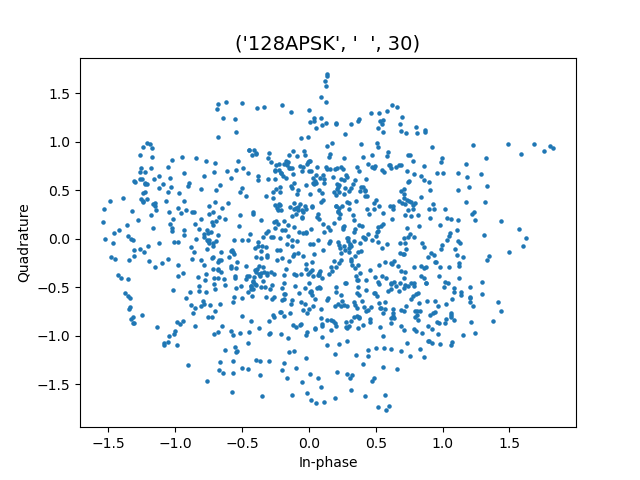
\includegraphics[width = 4.8cm]{/const/const_128APSK_30.png}} 
\subfloat{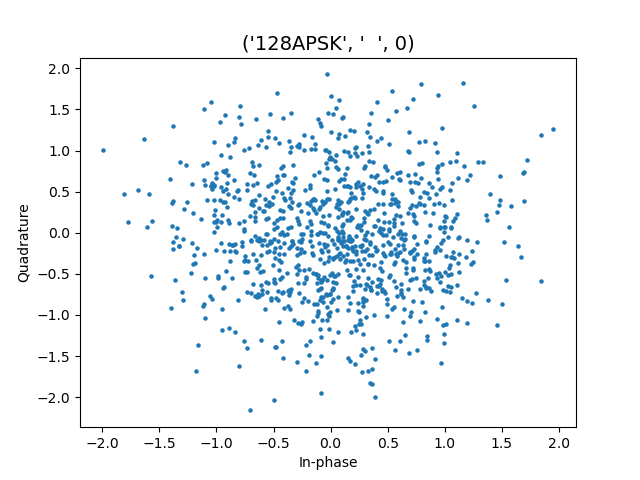
\includegraphics[width = 4.8cm]{/const/const_128APSK_0.png}}
\subfloat{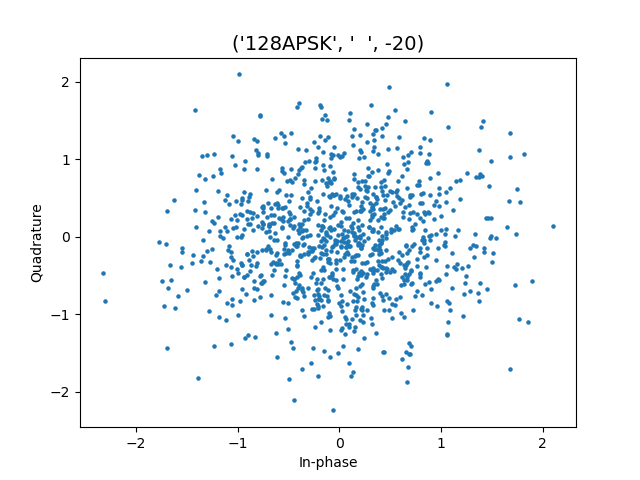
\includegraphics[width = 4.8cm]{/const/const_128APSK_-20.png}}\\
\caption{Sample Constellation Plots of Modulation modes 16PSK to 128APSK}
\label{Sample Const Plots 16PSK to 128APSK}
\vspace{-39pt}	 		
\end{figure*}

\begin{figure*}
\centering
\subfloat{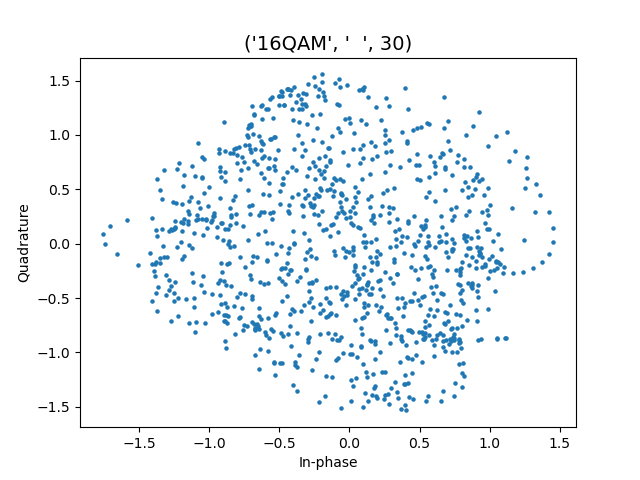
\includegraphics[width = 4.8cm]{/const/const_16QAM_30.png}} 
\subfloat{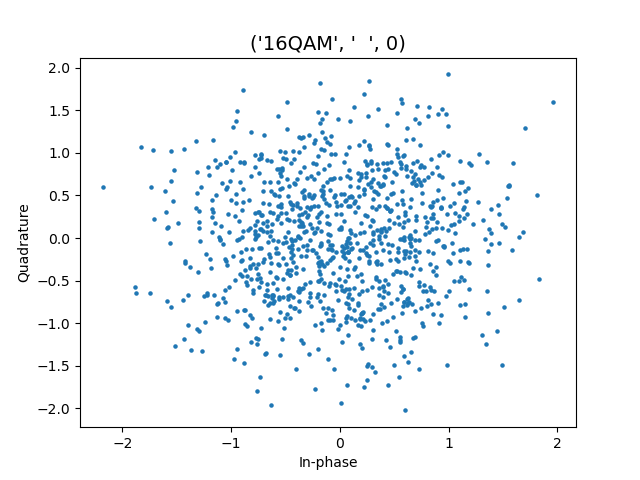
\includegraphics[width = 4.8cm]{/const/const_16QAM_0.png}}
\subfloat{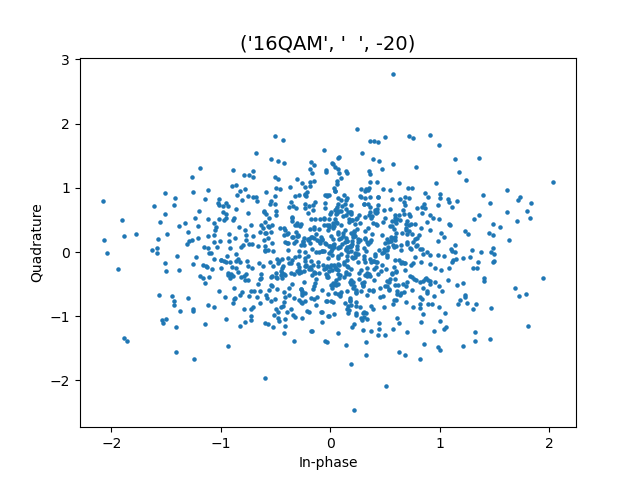
\includegraphics[width = 4.8cm]{/const/const_16QAM_-20.png}}\\
\subfloat{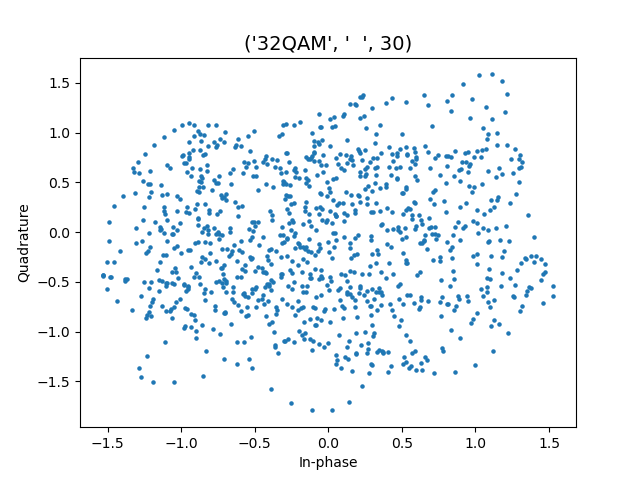
\includegraphics[width = 4.8cm]{/const/const_32QAM_30.png}} 
\subfloat{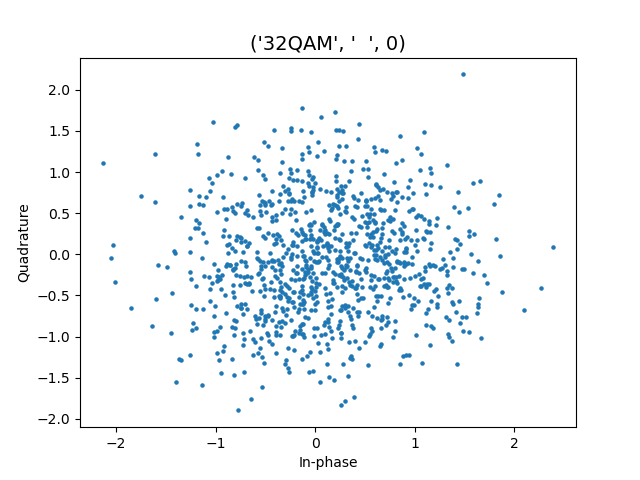
\includegraphics[width = 4.8cm]{/const/const_32QAM_0.png}}
\subfloat{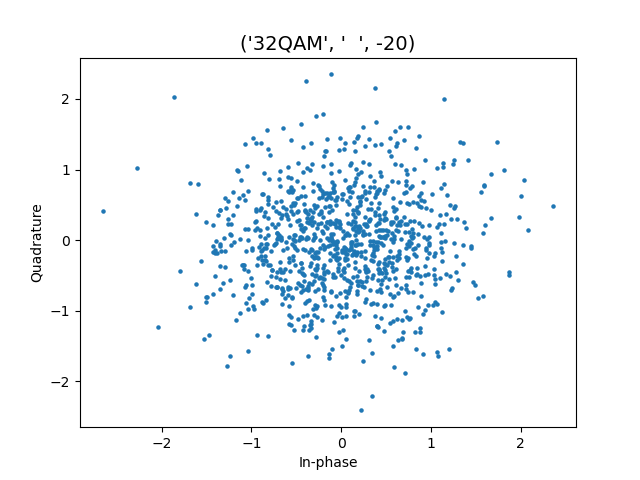
\includegraphics[width = 4.8cm]{/const/const_32QAM_-20.png}}\\
\subfloat{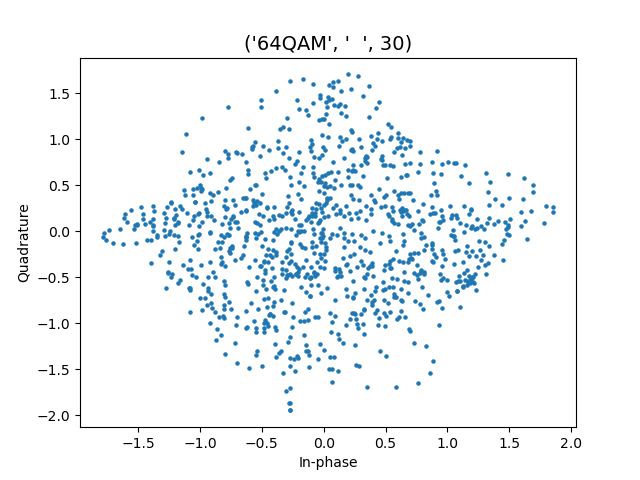
\includegraphics[width = 4.8cm]{/const/const_64QAM_30.png}} 
\subfloat{\includegraphics[width = 4.8cm]{/const/const_64QAM_0.png}}
\subfloat{\includegraphics[width = 4.8cm]{/const/const_64QAM_-20.png}}\\
\subfloat{\includegraphics[width = 4.8cm]{/const/const_128QAM_30.png}} 
\subfloat{\includegraphics[width = 4.8cm]{/const/const_128QAM_0.png}}
\subfloat{\includegraphics[width = 4.8cm]{/const/const_128QAM_-20.png}}\\
\subfloat{\includegraphics[width = 4.8cm]{/const/const_256QAM_30.png}} 
\subfloat{\includegraphics[width = 4.8cm]{/const/const_256QAM_0.png}}
\subfloat{\includegraphics[width = 4.8cm]{/const/const_256QAM_-20.png}}\\
\subfloat{\includegraphics[width = 4.8cm]{/const/const_AM-SSB-WC_30.png}} 
\subfloat{\includegraphics[width = 4.8cm]{/const/const_AM-SSB-WC_0.png}}
\subfloat{\includegraphics[width = 4.8cm]{/const/const_AM-SSB-WC_-20.png}}\\
\caption{Sample Constellation Plots of Modulation modes 32QAM to AM-SSB-WC}
\label{Sample Const Plots 16QAM to AM-SSB-WC}	 		
\vspace{-38pt}
\end{figure*}

\begin{figure*}
\centering
\subfloat{\includegraphics[width = 4.8cm]{/const/const_AM-SSB-SC_30.png}} 
\subfloat{\includegraphics[width = 4.8cm]{/const/const_AM-SSB-SC_0.png}}
\subfloat{\includegraphics[width = 4.8cm]{/const/const_AM-SSB-SC_-20.png}}\\
\subfloat{\includegraphics[width = 4.8cm]{/const/const_AM-DSB-WC_30.png}} 
\subfloat{\includegraphics[width = 4.8cm]{/const/const_AM-DSB-WC_0.png}}
\subfloat{\includegraphics[width = 4.8cm]{/const/const_AM-DSB-WC_-20.png}}\\
\subfloat{\includegraphics[width = 4.8cm]{/const/const_AM-DSB-SC_30.png}} 
\subfloat{\includegraphics[width = 4.8cm]{/const/const_AM-DSB-SC_0.png}}
\subfloat{\includegraphics[width = 4.8cm]{/const/const_AM-DSB-SC_-20.png}}\\
\subfloat{\includegraphics[width = 4.8cm]{/const/const_FM_30.png}} 
\subfloat{\includegraphics[width = 4.8cm]{/const/const_FM_0.png}}
\subfloat{\includegraphics[width = 4.8cm]{/const/const_FM_-20.png}}\\
\subfloat{\includegraphics[width = 4.8cm]{/const/const_GMSK_30.png}} 
\subfloat{\includegraphics[width = 4.8cm]{/const/const_GMSK_0.png}}
\subfloat{\includegraphics[width = 4.8cm]{/const/const_GMSK_-20.png}}\\
\subfloat{\includegraphics[width = 4.8cm]{/const/const_OQPSK_30.png}} 
\subfloat{\includegraphics[width = 4.8cm]{/const/const_OQPSK_0.png}}
\subfloat{\includegraphics[width = 4.8cm]{/const/const_OQPSK_-20.png}}\\
\caption{Sample Constellation Plots of Modulation modes AM-SSB-SC to OQPSK}
\label{Sample Const Plots AM-SSB-SC to OQPSK}	 		
\vspace{-26pt}
\end{figure*}

\begin{figure*}
\centering
\subfloat{\includegraphics[width = 4.5cm]{/IQ/IQ_OOK_30.png}} 
\subfloat{\includegraphics[width = 4.5cm]{/IQ/IQ_4ASK_30.png}}
\subfloat{\includegraphics[width = 4.5cm]{/IQ/IQ_8ASK_30.png}}
\subfloat{\includegraphics[width = 4.5cm]{/IQ/IQ_BPSK_30.png}}\\
\subfloat{\includegraphics[width = 4.5cm]{/IQ/IQ_QPSK_30.png}}
\subfloat{\includegraphics[width = 4.5cm]{/IQ/IQ_8PSK_30.png}} 
\subfloat{\includegraphics[width = 4.5cm]{/IQ/IQ_16PSK_30.png}}
\subfloat{\includegraphics[width = 4.5cm]{/IQ/IQ_32PSK_30.png}}\\
\subfloat{\includegraphics[width = 4.5cm]{/IQ/IQ_16APSK_30.png}}
\subfloat{\includegraphics[width = 4.5cm]{/IQ/IQ_32APSK_30.png}} 
\subfloat{\includegraphics[width = 4.5cm]{/IQ/IQ_64APSK_30.png}}
\subfloat{\includegraphics[width = 4.5cm]{/IQ/IQ_128APSK_30.png}}\\
\subfloat{\includegraphics[width = 4.5cm]{/IQ/IQ_16QAM_30.png}}
\subfloat{\includegraphics[width = 4.5cm]{/IQ/IQ_32QAM_30.png}} 
\subfloat{\includegraphics[width = 4.5cm]{/IQ/IQ_64QAM_30.png}}
\subfloat{\includegraphics[width = 4.5cm]{/IQ/IQ_128QAM_30.png}}\\
\subfloat{\includegraphics[width = 4.5cm]{/IQ/IQ_256QAM_30.png}}
\subfloat{\includegraphics[width = 4.5cm]{/IQ/IQ_AM-SSB-WC_30.png}} 
\subfloat{\includegraphics[width = 4.5cm]{/IQ/IQ_AM-SSB-SC_30.png}}
\subfloat{\includegraphics[width = 4.5cm]{/IQ/IQ_AM-DSB-WC_30.png}}\\
\subfloat{\includegraphics[width = 4.5cm]{/IQ/IQ_AM-DSB-SC_30.png}}
\subfloat{\includegraphics[width = 4.5cm]{/IQ/IQ_FM_30.png}} 
\subfloat{\includegraphics[width = 4.5cm]{/IQ/IQ_GMSK_30.png}}
\subfloat{\includegraphics[width = 4.5cm]{/IQ/IQ_OQPSK_30.png}}\\
\caption{Sample Plots of Modulation modes IQ captures}
\label{Sample Plots IQ captures}	 		
\vspace{-26pt}
\end{figure*}

\begin{figure*}
\centering
\subfloat{\includegraphics[width = 4.5cm]{/Mag/Mag_OOK_30.png}} 
\subfloat{\includegraphics[width = 4.5cm]{/Mag/Mag_4ASK_30.png}}
\subfloat{\includegraphics[width = 4.5cm]{/Mag/Mag_8ASK_30.png}}
\subfloat{\includegraphics[width = 4.5cm]{/Mag/Mag_BPSK_30.png}}\\
\subfloat{\includegraphics[width = 4.5cm]{/Mag/Mag_QPSK_30.png}}
\subfloat{\includegraphics[width = 4.5cm]{/Mag/Mag_8PSK_30.png}} 
\subfloat{\includegraphics[width = 4.5cm]{/Mag/Mag_16PSK_30.png}}
\subfloat{\includegraphics[width = 4.5cm]{/Mag/Mag_32PSK_30.png}}\\
\subfloat{\includegraphics[width = 4.5cm]{/Mag/Mag_16APSK_30.png}}
\subfloat{\includegraphics[width = 4.5cm]{/Mag/Mag_32APSK_30.png}} 
\subfloat{\includegraphics[width = 4.5cm]{/Mag/Mag_64APSK_30.png}}
\subfloat{\includegraphics[width = 4.5cm]{/Mag/Mag_128APSK_30.png}}\\
\subfloat{\includegraphics[width = 4.5cm]{/Mag/Mag_16QAM_30.png}}
\subfloat{\includegraphics[width = 4.5cm]{/Mag/Mag_32QAM_30.png}} 
\subfloat{\includegraphics[width = 4.5cm]{/Mag/Mag_64QAM_30.png}}
\subfloat{\includegraphics[width = 4.5cm]{/Mag/Mag_128QAM_30.png}}\\
\subfloat{\includegraphics[width = 4.5cm]{/Mag/Mag_256QAM_30.png}}
\subfloat{\includegraphics[width = 4.5cm]{/Mag/Mag_AM-SSB-WC_30.png}} 
\subfloat{\includegraphics[width = 4.5cm]{/Mag/Mag_AM-SSB-SC_30.png}}
\subfloat{\includegraphics[width = 4.5cm]{/Mag/Mag_AM-DSB-WC_30.png}}\\
\subfloat{\includegraphics[width = 4.5cm]{/Mag/Mag_AM-DSB-SC_30.png}}
\subfloat{\includegraphics[width = 4.5cm]{/Mag/Mag_FM_30.png}} 
\subfloat{\includegraphics[width = 4.5cm]{/Mag/Mag_GMSK_30.png}}
\subfloat{\includegraphics[width = 4.5cm]{/Mag/Mag_OQPSK_30.png}}\\
\caption{Sample Plots of Modulation modes IQ captures converted to magnitude}
\label{Sample Plots IQ captures converted to magnitude}	 		
\vspace{-26pt}
\end{figure*}

\begin{figure*}
\centering
\subfloat{\includegraphics[width = 4.5cm]{/UMAP/OOK_UMAP_Plot.png}} 
\subfloat{\includegraphics[width = 4.5cm]{/UMAP/4ASK_UMAP_Plot.png}}
\subfloat{\includegraphics[width = 4.5cm]{/UMAP/8ASK_UMAP_Plot.png}}
\subfloat{\includegraphics[width = 4.5cm]{/UMAP/BPSK_UMAP_Plot.png}}\\
\subfloat{\includegraphics[width = 4.5cm]{/UMAP/8PSK_UMAP_Plot.png}}
\subfloat{\includegraphics[width = 4.5cm]{/UMAP/QPSK_UMAP_Plot.png}} 
\subfloat{\includegraphics[width = 4.5cm]{/UMAP/16PSK_UMAP_Plot.png}}
\subfloat{\includegraphics[width = 4.5cm]{/UMAP/32PSK_UMAP_Plot.png}}\\
\subfloat{\includegraphics[width = 4.5cm]{/UMAP/16APSK_UMAP_Plot.png}}
\subfloat{\includegraphics[width = 4.5cm]{/UMAP/32APSK_UMAP_Plot.png}} 
\subfloat{\includegraphics[width = 4.5cm]{/UMAP/64APSK_UMAP_Plot.png}}
\subfloat{\includegraphics[width = 4.5cm]{/UMAP/128APSK_UMAP_Plot.png}}\\
\subfloat{\includegraphics[width = 4.5cm]{/UMAP/16QAM_UMAP_Plot.png}}
\subfloat{\includegraphics[width = 4.5cm]{/UMAP/32QAM_UMAP_Plot.png}} 
\subfloat{\includegraphics[width = 4.5cm]{/UMAP/64QAM_UMAP_Plot.png}}
\subfloat{\includegraphics[width = 4.5cm]{/UMAP/128QAM_UMAP_Plot.png}}\\
\subfloat{\includegraphics[width = 4.5cm]{/UMAP/256QAM_UMAP_Plot.png}}
\subfloat{\includegraphics[width = 4.5cm]{/UMAP/AM-SSB-WC_UMAP_Plot.png}} 
\subfloat{\includegraphics[width = 4.5cm]{/UMAP/AM-SSB-SC_UMAP_Plot.png}}
\subfloat{\includegraphics[width = 4.5cm]{/UMAP/AM-DSB-WC_UMAP_Plot.png}}\\
\subfloat{\includegraphics[width = 4.5cm]{/UMAP/AM-DSB-SC_UMAP_Plot.png}}
\subfloat{\includegraphics[width = 4.5cm]{/UMAP/FM_UMAP_Plot.png}} 
\subfloat{\includegraphics[width = 4.5cm]{/UMAP/GMSK_UMAP_Plot.png}}
\subfloat{\includegraphics[width = 4.5cm]{/UMAP/OQPSK_UMAP_Plot.png}}
\caption{UMAP Plots of Modulation modes in RadioML 2018 dataset}
\label{UMAP Plots}	 		
\end{figure*}

\begin{figure*}
\centering
\subfloat{\includegraphics[width = 4.5cm]{/UMAP/OOK_UMAP_Plot_noise.png}} 
\subfloat{\includegraphics[width = 4.5cm]{/UMAP/4ASK_UMAP_Plot_noise.png}}
\subfloat{\includegraphics[width = 4.5cm]{/UMAP/8ASK_UMAP_Plot_noise.png}}
\subfloat{\includegraphics[width = 4.5cm]{/UMAP/BPSK_UMAP_Plot_noise.png}}\\
\subfloat{\includegraphics[width = 4.5cm]{/UMAP/QPSK_UMAP_Plot_noise.png}}
\subfloat{\includegraphics[width = 4.5cm]{/UMAP/8PSK_UMAP_Plot_noise.png}} 
\subfloat{\includegraphics[width = 4.5cm]{/UMAP/16PSK_UMAP_Plot_noise.png}}
\subfloat{\includegraphics[width = 4.5cm]{/UMAP/32PSK_UMAP_Plot_noise.png}}\\
\subfloat{\includegraphics[width = 4.5cm]{/UMAP/16APSK_UMAP_Plot_noise.png}}
\subfloat{\includegraphics[width = 4.5cm]{/UMAP/32APSK_UMAP_Plot_noise.png}} 
\subfloat{\includegraphics[width = 4.5cm]{/UMAP/64APSK_UMAP_Plot_noise.png}}
\subfloat{\includegraphics[width = 4.5cm]{/UMAP/128APSK_UMAP_Plot_noise.png}}\\
\subfloat{\includegraphics[width = 4.5cm]{/UMAP/16QAM_UMAP_Plot_noise.png}}
\subfloat{\includegraphics[width = 4.5cm]{/UMAP/32QAM_UMAP_Plot_noise.png}} 
\subfloat{\includegraphics[width = 4.5cm]{/UMAP/64QAM_UMAP_Plot_noise.png}}
\subfloat{\includegraphics[width = 4.5cm]{/UMAP/128QAM_UMAP_Plot_noise.png}}\\
\subfloat{\includegraphics[width = 4.5cm]{/UMAP/256QAM_UMAP_Plot_noise.png}}
\subfloat{\includegraphics[width = 4.5cm]{/UMAP/AM-SSB-WC_UMAP_Plot_noise.png}} 
\subfloat{\includegraphics[width = 4.5cm]{/UMAP/AM-SSB-SC_UMAP_Plot_noise.png}}
\subfloat{\includegraphics[width = 4.5cm]{/UMAP/AM-DSB-WC_UMAP_Plot_noise.png}}\\
\subfloat{\includegraphics[width = 4.5cm]{/UMAP/AM-DSB-SC_UMAP_Plot_noise.png}}
\subfloat{\includegraphics[width = 4.5cm]{/UMAP/FM_UMAP_Plot_noise.png}} 
\subfloat{\includegraphics[width = 4.5cm]{/UMAP/GMSK_UMAP_Plot_noise.png}}
\subfloat{\includegraphics[width = 4.5cm]{/UMAP/OQPSK_UMAP_Plot_noise.png}}
\caption{UMAP Plots of Modulation modes with additive noise in RadioML 2018 dataset}
\label{UMAP Noise Plots}	 		
\end{figure*}

\onecolumn
\begin{table}
\centering
\caption{CHAODA AUC Scores -20 to 0 dB}
\begin{tabular}{|l|l|l|l|l|l|l|l|l|l|l|l|} 
\hline
     & \multicolumn{11}{c|}{\textbf{SNR (dB)}}                                                                                                                                                                                                                                                                                                                                 \\
\hline
\multicolumn{1}{|c|}{\textbf{Modulation}} & \multicolumn{1}{c|}{\textbf{-20}} & \multicolumn{1}{c|}{\textbf{-18}} & \multicolumn{1}{c|}{\textbf{-16}} & \multicolumn{1}{c|}{\textbf{-14}} & \multicolumn{1}{c|}{\textbf{-12}} & \multicolumn{1}{c|}{\textbf{-10}} & \multicolumn{1}{c|}{\textbf{-8}} & \multicolumn{1}{c|}{\textbf{-6}} & \multicolumn{1}{c|}{\textbf{-4}} & \multicolumn{1}{c|}{\textbf{-2}} & \multicolumn{1}{c|}{\textbf{0}}  \\ 
\hline OOK & 0.50  & 0.50 & 0.50  & 0.51  & 0.50  & 0.50  & 0.54  & 0.78 & 0.98  & 1.00 & 1.00\\ 
\hline 4ASK & 0.50   & 0.50  & 0.50  & 0.50   & 0.51  & 0.50  & 0.52 & 0.76 & 1.00 & 1.00 & 1.00\\ 
\hline 8ASK & 0.50 & 0.49 & 0.50 & 0.51 & 0.50 & 0.49 & 0.51 & 0.83 & 0.99 & 1.00 & 1.00\\ 
\hline BPSK & 0.51 & 0.50 & 0.50 & 0.49 & 0.50 & 0.51 & 0.50 & 0.49 & 0.50 & 0.50 & 0.53\\ 
\hline QPSK & 0.50 & 0.50 & 0.49 & 0.51 & 0.50 & 0.50 & 0.51  & 0.51  & 0.50  & 0.52 & 0.52\\ 
\hline 8PSK & 0.49 & 0.51 & 0.50 & 0.50 & 0.50 & 0.50 & 0.50 & 0.50 & 0.51 & 0.50 & 0.56\\ 
\hline 16PSK & 0.50 & 0.50 & 0.50 & 0.50 & 0.49 & 0.50 & 0.50 & 0.50 & 0.49 & 0.51 & 0.54\\ 
\hline 32PSK & 0.50 & 0.50 & 0.50 & 0.51 & 0.49 & 0.50 & 0.50 & 0.49 & 0.50 & 0.51 & 0.52\\ 
\hline 16APSK & 0.49 & 0.50 & 0.49 & 0.50 & 0.49 & 0.50 & 0.50 & 0.50 & 0.50 & 0.50 & 0.54\\ 
\hline 32APSK & 0.50 & 0.49 & 0.49 & 0.49 & 0.51 & 0.51 & 0.51 & 0.50 & 0.51 & 0.50 & 0.57\\ 
\hline 64APSK & 0.50 & 0.50 & 0.49 & 0.49 & 0.49 & 0.50 & 0.49 & 0.50 & 0.50 & 0.53 & 0.54\\ 
\hline 128APSK & 0.50 & 0.50 & 0.50 & 0.50 & 0.50 & 0.50 & 0.51 & 0.50 & 0.51 & 0.50 & 0.53\\ 
\hline 16QAM & 0.50 & 0.50 & 0.50 & 0.50 & 0.50 & 0.50 & 0.50 & 0.50 & 0.49 & 0.52 & 0.56\\ 
\hline 32QAM & 0.50 & 0.50 & 0.50 & 0.50 & 0.49 & 0.50 & 0.50 & 0.50 & 0.50 & 0.49 & 0.53\\ 
\hline 64QAM & 0.50 & 0.50 & 0.50 & 0.50 & 0.51 & 0.50 & 0.50 & 0.49 & 0.50 & 0.50 & 0.54\\ 
\hline 128QAM & 0.50 & 0.50 & 0.50 & 0.51 & 0.50 & 0.50 & 0.50 & 0.50 & 0.49 & 0.49 & 0.55\\ 
\hline 256QAM & 0.49 & 0.49 & 0.50 & 0.50 & 0.50 & 0.50 & 0.50 & 0.50 & 0.49 & 0.51 & 0.55\\ 
\hline AM-SSB-WC & 0.50 & 0.50 & 0.51 & 0.51 & 0.51 & 0.51 & 0.54 & 0.83 & 1.00 & 1.00 & 1.00\\ 
\hline AM-SSB-SC & 0.49 & 0.50 & 0.51 & 0.50 & 0.50 & 0.50 & 0.51 & 0.86 & 1.00 & 1.00 & 1.00 \\ 
\hline AM-DSB-WC & 0.50 & 0.50 & 0.50 & 0.49 & 0.50 & 0.50 & 0.52 & 0.51 & 0.51 & 0.49 & 0.61\\ 
\hline AM-DSB-SC & 0.50 & 0.50 & 0.50 & 0.49 & 0.50 & 0.51 & 0.51 & 0.52 & 0.53 & 0.63 & 0.79\\ 
\hline FM  & 0.50 & 0.51 & 0.51 & 0.51 & 0.50 & 0.49 & 0.50 & 0.51 & 0.50 & 0.51 & 0.58\\ 
\hline GMSK & 0.50 & 0.51 & 0.51 & 0.49 & 0.50 & 0.50 & 0.50 & 0.49 & 0.50 & 0.51 & 0.53\\ 
\hline OQPSK & 0.50 & 0.50 & 0.50 & 0.49 & 0.50 & 0.50 & 0.50 & 0.50 & 0.51 & 0.50 & 0.52\\
\hline
\end{tabular}
\label{CHAODA AUC Scores -20 to 0}
\end{table}

\begin{table}[H]
\centering
\caption{CHAODA AUC Scores 2 to 30 dB}
\begin{tabular}{|l|l|l|l|l|l|l|l|l|l|l|l|l|l|l|l|} 
\hline
     & \multicolumn{15}{c|}{\textbf{SNR (dB)}}                                                                                                                                                                                                                                                                                                                                                                                                                                                                    \\
\hline
\multicolumn{1}{|c|}{\textbf{Modulation}} & \multicolumn{1}{c|}{\textbf{2}} & \multicolumn{1}{c|}{\textbf{4}} & \multicolumn{1}{c|}{\textbf{6}} & \multicolumn{1}{c|}{\textbf{8}} & \multicolumn{1}{c|}{\textbf{10}} & \multicolumn{1}{c|}{\textbf{12}} & \multicolumn{1}{c|}{\textbf{14}} & \multicolumn{1}{c|}{\textbf{16}} & \multicolumn{1}{c|}{\textbf{18}} & \multicolumn{1}{c|}{\textbf{20}} & \multicolumn{1}{c|}{\textbf{22}} & \multicolumn{1}{c|}{\textbf{24}} & \multicolumn{1}{c|}{\textbf{26}} & \multicolumn{1}{c|}{\textbf{28}} & \multicolumn{1}{c|}{\textbf{30}}  \\ 
\hline OOK  & 1.00 & 1.00 & 1.00 & 1.00 & 1.00 & 1.00 & 1.00 & 1.00 & 1.00 & 1.00 & 1.00 & 1.00 & 1.00 & 1.00 & 1.00 \\
\hline 4ASK & 1.00 & 1.00 & 1.00 & 1.00 & 1.00 & 1.00 & 1.00 & 1.00 & 1.00 & 1.00 & 1.00 & 1.00 & 1.00 & 1.00 & 1.00 \\
\hline 8ASK & 1.00 & 1.00 & 1.00 & 1.00 & 1.00 & 1.00 & 1.00 & 1.00 & 1.00 & 1.00 & 1.00 & 1.00 & 1.00 & 1.00 & 1.00 \\
\hline BPSK & 0.59 & 0.68 & 0.74 & 0.75 & 0.69 & 0.87 & 0.77 & 0.82 & 0.76 & 0.72 & 0.86 & 0.82 & 0.88 & 0.78 & 0.71 \\
\hline QPSK & 0.55 & 0.65 & 0.73 & 0.72 & 0.72 & 0.73 & 0.72 & 0.71 & 0.70 & 0.72 & 0.75 & 0.74 & 0.70 & 0.74 & 0.75 \\
\hline 8PSK & 0.55 & 0.58 & 0.63 & 0.59 & 0.62 & 0.65 & 0.65 & 0.68 & 0.67 & 0.66 & 0.59 & 0.66 & 0.67 & 0.65 & 0.68 \\
\hline 16PSK & 0.56 & 0.65 & 0.61 & 0.65 & 0.69 & 0.60 & 0.61 & 0.68 & 0.64 & 0.65 & 0.63 & 0.72 & 0.63 & 0.62 & 0.61 \\
\hline 32PSK & 0.55 & 0.60 & 0.58 & 0.67 & 0.64 & 0.66 & 0.67 & 0.63 & 0.63 & 0.65 & 0.72 & 0.63 & 0.70 & 0.63 & 0.66 \\
\hline 16APSK & 0.60 & 0.69 & 0.65 & 0.79 & 0.75 & 0.81 & 0.75 & 0.77 & 0.80 & 0.73 & 0.76 & 0.76 & 0.80 & 0.76 & 0.71 \\
\hline 32APSK & 0.68 & 0.83 & 0.85 & 0.83 & 0.83 & 0.92 & 0.85 & 0.91 & 0.87 & 0.85 & 0.87 & 0.88 & 0.89 & 0.86 & 0.85 \\
\hline 64APSK & 0.67 & 0.72 & 0.82 & 0.86 & 0.85 & 0.76 & 0.80 & 0.81 & 0.82 & 0.80 & 0.87 & 0.84 & 0.78 & 0.76 & 0.86 \\
\hline 128APSK & 0.64 & 0.76 & 0.86 & 0.84 & 0.82 & 0.83 & 0.83 & 0.84 & 0.86 & 0.85 & 0.84 & 0.84 & 0.84 & 0.79 & 0.89 \\
\hline 16QAM  & 0.70 & 0.80 & 0.83 & 0.84 & 0.83 & 0.79 & 0.85 & 0.89 & 0.85 & 0.81 & 0.84 & 0.88 & 0.87 & 0.85 & 0.82 \\
\hline 32QAM  & 0.72 & 0.77 & 0.78 & 0.82 & 0.85 & 0.83 & 0.87 & 0.85 & 0.87 & 0.81 & 0.87 & 0.84 & 0.83 & 0.87 & 0.85 \\
\hline 64QAM  & 0.63 & 0.81 & 0.74 & 0.85 & 0.79 & 0.80 & 0.82 & 0.83 & 0.85 & 0.85 & 0.81 & 0.87 & 0.92 & 0.86 & 0.77 \\
\hline 128QAM & 0.70 & 0.72 & 0.82 & 0.79 & 0.82 & 0.88 & 0.88 & 0.82 & 0.86 & 0.86 & 0.83 & 0.84 & 0.87 & 0.84 & 0.82 \\
\hline 256QAM & 0.62 & 0.80 & 0.86 & 0.83 & 0.88 & 0.85 & 0.84 & 0.83 & 0.92 & 0.81 & 0.90 & 0.92 & 0.87 & 0.83 & 0.84 \\
\hline AM-SSB-WC & 1.00 & 1.00 & 1.00 & 1.00 & 1.00 & 1.00 & 1.00 & 1.00 & 1.00 & 0.99 & 1.00 & 1.00 & 1.00 & 1.00 & 0.99 \\
\hline AM-SSB-SC & 1.00 & 1.00 & 1.00 & 1.00 & 1.00 & 1.00 & 1.00 & 1.00 & 1.00 & 1.00 & 1.00 & 1.00 & 1.00 & 1.00 & 1.00 \\
\hline AM-DSB-WC & 0.90 & 0.58 & 0.63 & 0.63 & 0.77 & 0.57 & 0.72 & 0.78 & 0.67 & 0.53 & 0.81 & 0.90 & 0.59 & 0.86 & 0.78 \\
\hline AM-DSB-SC & 0.95 & 1.00 & 1.00 & 1.00 & 0.99 & 1.00 & 0.98 & 0.99 & 0.99 & 0.84 & 0.92 & 0.96 & 0.99 & 0.98 & 0.97 \\
\hline FM & 0.50 & 0.61 & 0.56 & 0.52 & 0.52 & 0.57 & 0.52 & 0.58 & 0.55 & 0.59 & 0.55 & 0.56 & 0.53 & 0.46 & 0.58 \\
\hline GMSK & 0.57 & 0.56 & 0.60 & 0.66 & 0.62 & 0.66 & 0.64 & 0.64 & 0.67 & 0.69 & 0.69 & 0.71 & 0.65 & 0.73 & 0.67 \\
\hline OQPSK & 0.55 & 0.59 & 0.61  & 0.61  & 0.64  & 0.63 & 0.66  & 0.65 & 0.64  & 0.63 & 0.62 & 0.60 & 0.63  & 0.65  & 0.63\\
\hline
\end{tabular}
\label{CHAODA AUC Scores 2 to 30}
\end{table}
\end{document}
